% !TEX encoding = UTF-8 Unicode
% CDSL@UoS template: 4:3, boxes, 10pt, serif math, original logos and margins.
\documentclass[t,10pt,handout]{beamer}
% Original CDSL@UoS preamble, with class/note mode in main.tex.
% This is a basic template for H. Shim
% Aug. 19, 2008
% Modified by G. Park
% Sept. 20, 2023

% 제출해야할 때 handout 옵션 추가 발표할 때는 제거. 발표할 때 \pause 효과를 사용 할 수 있게 됨


  
\def\mynote{aa}   % Comment if mynote wants to appear

\mode<presentation>
{
  \usetheme{boxes}
  \usefonttheme[onlymath]{serif}
  \setbeamercovered{transparent}
}

\setbeamertemplate{navigation symbols}{}
% removes the navigation symbols
\setbeamertemplate{footline}[frame number]
%\setbeamertemplate{footline}[text line]{%
%color setting more or less matching U of A colors
%\setbeamercolor*{palette secondary}{use=structure,fg=white,bg=structure.fg!55!black}
%\setbeamercolor*{palette tertiary}{use=structure,fg=white,bg=red!50!black}

\usepackage{kotex}
\usepackage[english]{babel}
\usepackage[T1]{fontenc}
\usepackage{comment}
\usepackage{mathtools}
\usepackage{setspace}

\colorlet{Darkred}{red!50!black}
\colorlet{Darkgreen}{green!50!black}
\colorlet{Darkblue}{blue!70!black}
\newcommand{\colb}{\color{Darkblue}}
\newcommand{\colgr}{\color{gray}}
\newcommand{\colg}{\color{Darkgreen}}
\newcommand{\colr}{\color{Darkred}}

% Define Environment:
\newtheorem{thm}{\bf Theorem}
\newtheorem{prop}{\bf Proposition}
\newtheorem{lem}{\bf Lemma}
\newtheorem{assmpt}{\bf Assumption}
\newtheorem{defn}{\bf Definition}
\newtheorem{exmp}{\bf Example}
\newtheorem{cor}{\bf Corollary}
\newtheorem{condi}{\bf Condition}
%=== Non-italic Theorem Environment by Vin
\newtheorem{rem1}{\bf Remark}
\newenvironment{rem}{\begin{rem1}\normalfont}{\end{rem1}}
%=== New Example Environment by Vin
\newcounter{Examp}
\newenvironment{exam}{\stepcounter{Examp} \medskip \noindent {\bf Example \arabic{Examp}.}}{ \medskip }

%=== New Example Environment by Vin
\newcounter{exer}
\newenvironment{exer}{\stepcounter{exer} \medskip \noindent {\bf Exercise \arabic{exer}.}}{ \medskip }


% Define Some Notation:

\newcommand{\nn}{{\mathfrak{n}}}

\newcommand{\R}{\ensuremath{{\mathbb R}}}
\newcommand{\Z}{\ensuremath{{\mathbb Z}}}
\newcommand{\N}{\ensuremath{{\mathbb N}}}

\newcommand{\AAA}{{\mathcal A}}
\newcommand{\CC}{{\mathcal C}}
\newcommand{\DD}{{\mathcal D}}
\newcommand{\EE}{{\mathcal E}}
\newcommand{\FF}{{\mathcal F}}
\newcommand{\KK}{{\mathcal K}}
\newcommand{\LL}{{\mathcal L}}
\newcommand{\MM}{{\mathcal M}}
\newcommand{\NN}{{\mathcal N}}
\newcommand{\OO}{{\mathcal O}}
\newcommand{\PP}{{\mathcal P}}
\newcommand{\QQ}{{\mathcal Q}}
\newcommand{\RR}{{\mathcal R}}
\newcommand{\SSS}{{\mathcal S}}
\newcommand{\TT}{{\mathcal T}}
\newcommand{\UU}{{\mathcal U}}
\newcommand{\VV}{{\mathcal V}}
\newcommand{\WW}{{\mathcal W}}
\newcommand{\XX}{{\mathcal X}}
\newcommand{\YY}{{\mathcal Y}}
\newcommand{\cN}{\ensuremath{\mathcal{N}}}

\newcommand{\KL}{{\mathcal{KL}}}
\newcommand{\sat}{\ensuremath{{\rm sat}}}

\newcommand{\triend}{\hfill \ensuremath{\lhd}}
\DeclareMathOperator{\rank}{rank}

\newcommand{\cvector}[1]{\left(\!\!\!\begin{array}{c} #1 \end{array}\!\!\!\right)}
\newcommand{\setdef}[2]{\left\{\ #1\ \left|\ #2\ \right.\right\}}

\setbeamertemplate{itemize subitem}[circle]

\setstretch{1.1}

\setbeamersize{text margin left=0.5cm}  % <- like this
\setbeamersize{text margin right=0.5cm} % <- like this



\usepackage{booktabs,tabularx,bm,tikz,lmodern,appendixnumberbeamer}
\usetikzlibrary{arrows.meta,positioning,calc,fit,backgrounds,shapes.geometric}
\graphicspath{{Fig/}}
\definecolor{Accent}{HTML}{205493}
\definecolor{Success}{HTML}{28735E}
\definecolor{Muted}{HTML}{67727D}
\definecolor{Soft}{HTML}{F0F4F8}
% Saturated text emphasis, separate from structural and plot colors.
\definecolor{EmphasisRed}{HTML}{FF0000}
\definecolor{EmphasisBlue}{HTML}{0000FF}
\definecolor{EmphasisGreen}{HTML}{008000}
\definecolor{EmphasisOrange}{HTML}{E66A00}
\setbeamercolor{structure}{fg=Accent}
\setbeamercolor{block title}{fg=Soft,bg=Accent}
\setbeamercolor{block body}{fg=black,bg=Soft}
\setbeamercolor{alerted text}{fg=EmphasisRed}
\setbeamerfont{frametitle}{size=\fontsize{14.4}{17.3}\selectfont}
\setbeamerfont{title}{size=\fontsize{14.4}{17.3}\selectfont}
\setbeamerfont{subtitle}{size=\normalsize}
\setbeamerfont{framesubtitle}{size=\normalsize}
\setbeamercolor{framesubtitle}{fg=Accent}
\setbeamertemplate{bibliography item}[text]
\setbeamertemplate{bibliography entry title}{}
\setbeamertemplate{bibliography entry location}{}
\setbeamertemplate{bibliography entry note}{}
\setbeamerfont{block title}{size=\normalsize}
\setbeamertemplate{itemize item}{\color{Accent}$\blacktriangleright$}
\setlength{\tabcolsep}{5pt}
\pdfstringdefDisableCommands{\def\\{ }}

\newcommand{\takeaway}[1]{\par\begin{beamercolorbox}[sep=2mm,wd=\linewidth]{block body}\color{black}\textbf{#1}\end{beamercolorbox}\par\vspace{2mm}}
\newcommand{\ee}{\mathrm{ee}}
\newcommand{\regtask}{\mathbf{T}_{\ee}}
\newcommand{\subtask}[1]{\mathbf{ST}_{\ee,#1}}
\newcommand{\qstar}{q^*}
\newcommand{\norm}[1]{\left\lVert#1\right\rVert}
\DeclareMathOperator*{\argmax}{arg\,max}
\DeclareMathOperator*{\argmin}{arg\,min}
\tikzset{box/.style={draw=Accent!60,fill=Soft,rounded corners=2pt,align=center,
    minimum height=10mm,inner sep=3mm,font=\normalsize},
    arr/.style={-{Stealth[length=2mm]},thick,draw=Accent},
    mini/.style={box,font=\normalsize,inner sep=2mm,minimum height=8mm}}

% Author verified against the user's sequential-safety-IK manuscript.
% Defense date is deliberately blank; set it here when the date is fixed.
\title{Collision-Aware Sequential Kinematic Control of Robot Manipulators Using Control Barrier Functions and Supervised Learning-based Task Sequencing}
\subtitle{Master's Thesis Defense}
\author{Jinwoo Lee\\[1.5mm]\normalsize Advisor: Gyunghoon Park}
\institute{\normalsize Department of Electrical and Computer Engineering\\University of Seoul\\[1mm]
  \normalsize Control \& Dynamic Systems Lab.\\[1mm]
  
\includegraphics[height=12mm]{CDSLlogo.png}\hspace{6mm}
\includegraphics[height=12mm]{UoSlogo.jpg}}
\date{}
\hypersetup{pdftitle={Collision-Aware Sequential Kinematic Control of Robot Manipulators Using Control Barrier Functions and Supervised Learning-based Task Sequencing},pdfauthor={Jinwoo Lee},pdfsubject={20-minute English Master's Thesis Defense}}


% Consistent slide rhythm: fixed content area with flexible gaps between groups.
\newenvironment{slidebody}{\begin{minipage}[t][68.5mm][s]{\linewidth}\vspace{0pt}}{\par\vspace{0pt}\end{minipage}}
\newcommand{\appendixentry}[2]{%
  \noindent\hyperlink{appendix-a#1}{\strut\makebox[8mm][l]{\color{Accent}\textbf{A#1}}#2}\par\vspace{.2mm}}
\newcommand{\metricbox}[3]{%
  \begin{beamercolorbox}[wd=\linewidth,ht=4mm,dp=4mm,center]{block title}\normalsize #1\end{beamercolorbox}%
  \nointerlineskip
  \begin{beamercolorbox}[wd=\linewidth,ht=13mm,dp=3mm,center]{block body}%
    {\normalsize #2}\\[2mm]{\normalsize #3}%
  \end{beamercolorbox}}


% Consecutive frames share a fixed diagram viewport (handout-safe progression).
\newcommand{\selectorfigure}[1]{%
  \begin{tikzpicture}[x=1mm,y=1mm,
      compact/.style={mini,anchor=north,font=\normalsize,inner sep=.8mm,minimum height=6.5mm},
      flow/.style={compact,anchor=center,text width=30mm,minimum height=7.5mm}]
    \path[use as bounding box] (-57,-55.5) rectangle (57,1);
    \node[compact,text width=44mm,minimum height=10mm](r) at (-27,0){Start, IK, and goal inputs\\$q_0,q^*,p_{\mathrm d},R_{\mathrm d}$};
    \node[compact,text width=44mm,minimum height=10mm](o) at (27,0){Obstacle set $\mathcal O$\\$(c_x,c_y,c_z,r)$};
    \node[compact,text width=44mm](re) at (-27,-12){Robot \& goal encoder};
    \node[compact,text width=44mm](oe) at (27,-12){Common obstacle encoder};
    \node[compact,text width=80mm,minimum height=10mm](a) at (0,-22){\textcolor{EmphasisRed}{\textbf{Cross-attention}}~\cite{vaswani2017attention}\\Robot \& goal query / obstacle keys and values};
    \ifnum#1=1
      \node[compact,text width=80mm](h) at (0,-35){Success scores $\hat p_k$ for 10 pairs};
      \node at (0,-49){$z=(q_0,q^*,p_{\mathrm d},R_{\mathrm d},\mathcal O)$};
    \else
      \node[compact,text width=80mm](h) at (0,-35){Success scores $\hat p_k$ $\to$ selected pair $S_{\hat k(z)}$};
    \fi
    \draw[arr](r.south)--(re.north);
    \draw[arr](o.south)--(oe.north);
    \draw[arr](re.south)--(re.south |- a.north);
    \draw[arr](oe.south)--(oe.south |- a.north);
    \draw[arr](a.south)--(h.north);
    \coordinate (bypass) at (-55,0);
    \draw[arr,rounded corners=1mm](re.west)--(bypass |- re.west)--(bypass |- h.west)--(h.west);
    \ifnum#1=2
      \node[flow,font=\fontsize{10}{10}\selectfont,inner ysep=.4mm](seq) at (-38,-50.75){Subtask targets\\and sequence};
      \node[flow](qp) at (0,-50.75){CLF--CBF QP};
      \node[flow](u) at (38,-50.75){Joint velocity $u$};
      \coordinate (routing) at (0,-44);
      \draw[arr,rounded corners=.6mm](h.south)--(routing)--(routing -| seq.north)--(seq.north);
      \draw[arr](seq.east)--(qp.west);
      \draw[arr](qp.east)--(u.west);
    \fi
  \end{tikzpicture}}

% Fixed image size and origin across the five Planar explanation frames.
\newcommand{\planarstage}[2]{%
  \begin{columns}[c,onlytextwidth]
    \column{.40\textwidth}
    \begin{minipage}[c][64mm][c]{\linewidth}\centering
      \includegraphics[width=\linewidth]{#1}
    \end{minipage}
    \column{.58\textwidth}
    \begin{minipage}[c][64mm][c]{\linewidth}\centering
      #2
    \end{minipage}
  \end{columns}}

\newcommand{\taskqp}[3]{%
  {\color{#2}$\subtask{#1}\ifnum#1=3=\regtask\fi\;\longrightarrow\;\mathrm{QP}_{#1}$}\par
  \[\begin{gathered}
    \min_{u,\delta}\quad \tfrac12u^\top W_{\mathrm{u}} u+\tfrac12w_\delta\delta^2\\[2mm]
    \text{s.t.}\quad {\color{#2}\nabla_q V_{#1}^{\top}u\leq-#3V_{#1}+\delta}\\[2mm]
    \nabla_qh_r^\top u\geq-\gamma_r h_r,\quad r=1,\ldots,B\\[2mm]
    -\alpha_j(q_j-q_{j,\min})\leq u_j\leq\alpha_j(q_{j,\max}-q_j)\\[2mm]
    v_{\min,j}\leq u_j\leq v_{\max,j},\quad j=1,\ldots,n
  \end{gathered}\]}

\newcommand{\sequentialframework}{%
    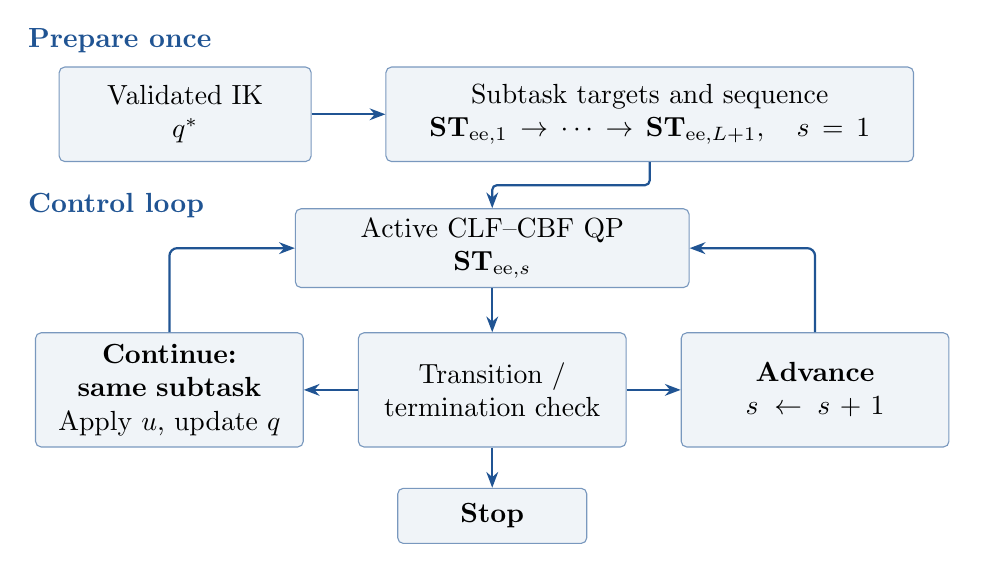
\begin{tikzpicture}[x=1mm,y=-1mm,
        flow/.style={box,inner sep=1mm,minimum height=12mm},
        phase/.style={font=\normalsize\bfseries,text=Accent,anchor=north west,inner sep=0pt}]
      \path[use as bounding box](0,0)rectangle(118,66);
      \node[phase] at(0,0){Prepare once};
      \node[flow,text width=30mm](ik)at(20,11){Validated IK\\$q^*$};
      \node[flow,text width=65mm](setup)at(79,11){Subtask targets and sequence\\$\subtask{1}\to\cdots\to\subtask{L+1},\quad s=1$};
      \draw[arr](ik.east)--(setup.west);
      \node[phase] at(0,21){Control loop};
      \node[flow,text width=48mm,minimum height=10mm](qp)at(59,28){Active CLF--CBF QP\\$\subtask{s}$};
      \draw[arr,rounded corners=.6mm](setup.south)--(79,20)--(59,20)--(qp.north);
      \node[flow,text width=32mm,minimum height=14.5mm](check)at(59,46){Transition /\\termination check};
      \node[flow,text width=32mm,minimum height=14.5mm](apply)at(18,46){\textbf{Continue: same subtask}\\Apply $u$, update $q$};
      \node[flow,text width=32mm,minimum height=14.5mm](advance)at(100,46){\textbf{Advance}\\$s\leftarrow s+1$};
      \node[flow,text width=22mm,minimum height=7mm](stop)at(59,62){\textbf{Stop}};
      \draw[arr](qp.south)--(check.north);
      \draw[arr](check.west)--(apply.east);
      \draw[arr](check.east)--(advance.west);
      \draw[arr](check.south)--(stop.north);
      \draw[arr,rounded corners=1mm](apply.north)--(18,28)--(qp.west);
      \draw[arr,rounded corners=1mm](advance.north)--(100,28)--(qp.east);
    \end{tikzpicture}}

% Section labels and one dot per main slide, following the reference deck.
% Completed: filled gray. Current: larger blue. Upcoming: hollow gray.
% The cover is excluded; backup slides have an independent page count.
\makeatletter
\providecommand{\DefenseProgressStage}{}
\newcommand{\defensepart}[1]{\gdef\DefenseProgressStage{#1}}
% Generated by scripts/build_progress_data.py from evidence/story_plan.json.
% One dot per main slide; the cover and backup slides are excluded.
\newcommand{\DefenseProgressGroups}{%
  \defense@group{Motivation}{2}{3}%
  \defense@group{Background}{4}{7}%
  \defense@group{Planar}{8}{19}%
  \defense@group{Spatial}{20}{26}%
  \defense@group{Learning}{27}{30}%
  \defense@group{Results}{31}{36}%
}


\newcommand{\defense@group}[3]{%
  \def\defense@width{15mm}%
  \def\defense@candidate{#1}%
  \def\defense@name{Motivation}\ifx\defense@candidate\defense@name\def\defense@width{20mm}\fi
  \def\defense@name{Background}\ifx\defense@candidate\defense@name\def\defense@width{22mm}\fi
  \def\defense@name{Learning}\ifx\defense@candidate\defense@name\def\defense@width{17mm}\fi
  \makebox[\defense@width][c]{%
    \begin{tikzpicture}[x=1mm,y=1mm,baseline=0mm]
      \path[use as bounding box] (-8.5,0) rectangle (8.5,4);
      \def\defense@candidate{#1}%
      \ifx\DefenseProgressStage\defense@candidate
        \node[anchor=base,inner sep=0pt,font=\bfseries,text=Accent] at (0,2.02) {#1};
      \else
        \node[anchor=base,inner sep=0pt,text=black!75] at (0,2.02) {#1};
      \fi
      \foreach \defense@page in {#2,...,#3}{%
        \pgfmathsetmacro{\defense@x}{(\defense@page-(#2+#3)/2)*1.4}%
        \ifnum\defense@page<\c@framenumber
          \fill[black!55] (\defense@x,.65) circle[radius=.38];
        \else\ifnum\defense@page=\c@framenumber
          \fill[Accent] (\defense@x,.65) circle[radius=.55];
        \else
          \draw[black!45,line width=.25pt] (\defense@x,.65) circle[radius=.38];
        \fi\fi
      }%
    \end{tikzpicture}}}

\setbeamertemplate{footline}{%
  \leavevmode
  \begingroup
  \normalfont\fontsize{10}{12}\selectfont
  % Beamer adds 4 pt: the complete footer reserves less than 6.7 mm.
  \vbox to 5.2mm{%
    \offinterlineskip
    \hbox to \paperwidth{%
      \hskip5mm%
      \ifbeamer@inappendix
        \vrule width0pt height4mm depth0pt%
        \raisebox{1.6mm}{\makebox[\dimexpr\paperwidth-24mm\relax][l]{\hyperlink{appendix-contents}{\color{Accent}Appendix contents}}}%
        \raisebox{1.6mm}{\makebox[14mm][r]{\fontsize{7}{8.4}\selectfont\color{black!75}\insertframenumber\,/\,\inserttotalframenumber}}%
      \else
        \DefenseProgressGroups%
        \raisebox{1.6mm}{\makebox[14mm][r]{\fontsize{7}{8.4}\selectfont\color{black!75}\insertframenumber\,/\,\insertmainframenumber}}%
      \fi
      \hskip5mm\hss%
    }%
    \vskip.8mm
  }%
  \endgroup
}
\makeatother


\begin{document}

\begin{frame}[plain,label=title]
  \titlepage
\end{frame}

\defensepart{Motivation}

\begin{frame}[label=motivation-goal]{Why Safe Goal Reaching Matters}
  \framesubtitle{1.1 Research Background}
  \begin{slidebody}
    \centering
    \textbf{Example: A mobile robotic chemist}~\cite{burger2020chemist}\par\vspace{3mm}
    \begin{columns}[t,onlytextwidth]
      \column{.485\textwidth}\centering
      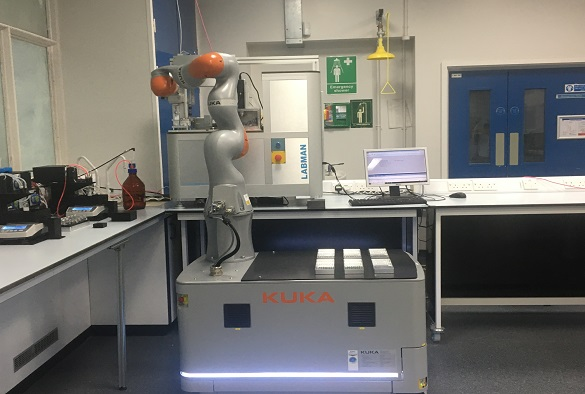
\includegraphics[width=\linewidth,height=37mm,keepaspectratio]{motivation_liverpool_lab.jpg}\par\vspace{2mm}
      Laboratory workspace
      \column{.485\textwidth}\centering
      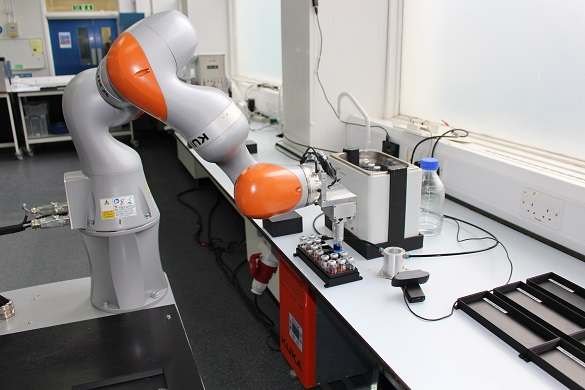
\includegraphics[width=\linewidth,height=37mm,keepaspectratio]{motivation_liverpool_handling.jpg}\par\vspace{2mm}
      Sample handling
    \end{columns}\par\vspace{3mm}
    {\fontsize{7}{8.5}\selectfont\href{https://www.liverpool.ac.uk/cooper-group/news/stories/title,1215738,en.php}{Photos: University of Liverpool}\par}\vfill
    \textbf{Safe reaching enables reliable task execution}\par\vfill
  \end{slidebody}
\end{frame}

\begin{frame}[label=motivation]{Safe Motion in Cluttered Workspaces}
  \framesubtitle{1.1 Research Background}
  \begin{slidebody}
    \takeaway{Safe goal reaching requires whole-arm collision avoidance.}

    \begin{columns}[c,onlytextwidth]
      \column{.67\textwidth}\centering
      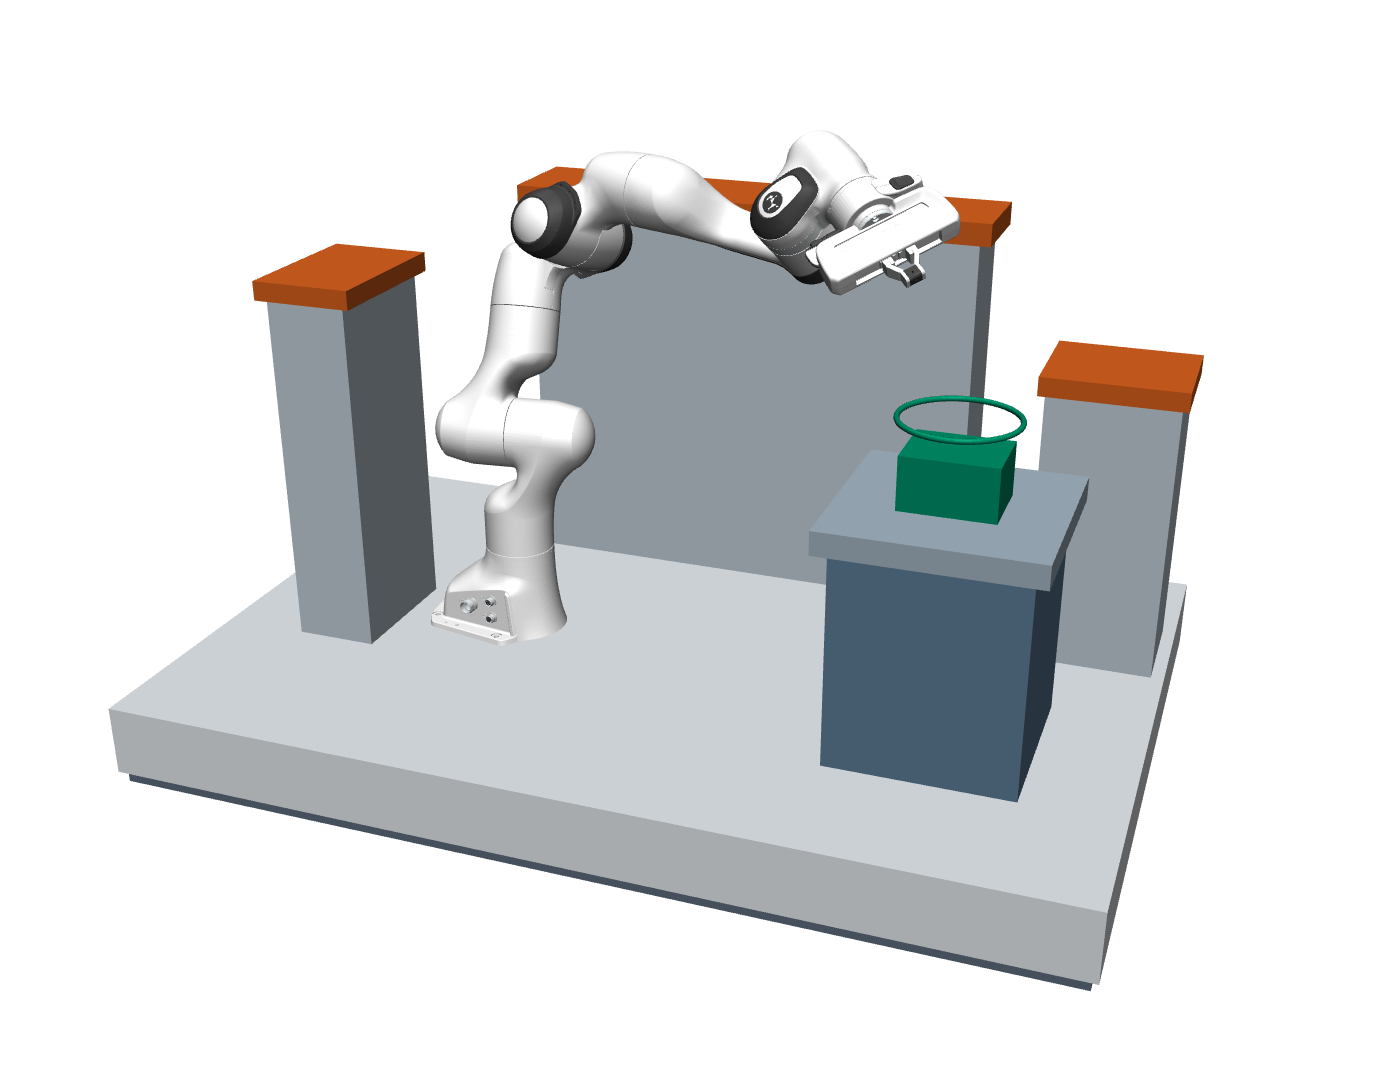
\includegraphics[width=\linewidth,height=53mm,keepaspectratio]{motivation_safety.png}
      \column{.30\textwidth}
      \textbf{Goal reaching}\par\vspace{2mm}
      Reach the target pose\par\vspace{6mm}
      \textbf{Collision avoidance}\par\vspace{2mm}
      Keep every link clear of obstacles
    \end{columns}
  \end{slidebody}
\end{frame}

\defensepart{Background}

\begin{frame}[label=background-clf]{Kinematic Control and Goal-Error Reduction}
  \framesubtitle{2.1 Control Lyapunov Function}
  \begin{slidebody}
    \centering
    \textbf{Kinematic control: joint velocity as the input}\par\vspace{2mm}
    $\dot q=u,\quad q:\ \text{joint angles},\quad u:\ \text{joint velocity}$\par\vspace{3mm}
    \begin{columns}[c,onlytextwidth]
      \column{.49\textwidth}\centering
      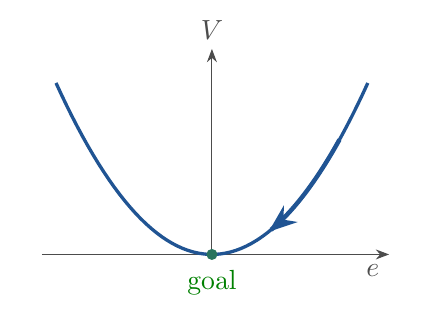
\begin{tikzpicture}[x=9mm,y=9mm]
        \path[use as bounding box] (-2.6,-.7) rectangle (2.6,3.2);
        \draw[-{Stealth},black!70](-2.4,0)--(2.5,0) node[below left]{$e$};
        \draw[-{Stealth},black!70](0,0)--(0,2.9) node[above]{$V$};
        \draw[Accent,line width=1.2pt,domain=-2.2:2.2,samples=60] plot(\x,{.5*\x*\x});
        \draw[Accent,line width=1.6pt,-{Stealth},domain=1.8:.8,samples=30] plot(\x,{.5*\x*\x});
        \fill[Success](0,0)circle(2pt);
        \node[text=EmphasisGreen,below]at(0,-.08){goal};
      \end{tikzpicture}
      \column{.47\textwidth}\raggedright
      \begin{tabular}{@{}l@{}}
        \textbf{Control Lyapunov Function}         \\[1mm]
        $\displaystyle V(q)=\tfrac12\norm{e(q)}^2$ \\[1mm]
        $e(q)$: task error                         \\[5mm]
        \textbf{CLF constraint}                    \\[1mm]
        $\displaystyle\dot V=\nabla_qV^\top u\leq-c_VV,\quad c_V>0$
      \end{tabular}
    \end{columns}
    \vfill
    $V=0$: task satisfied\qquad $\dot V<0$: error reduction\par
    \vfill
  \end{slidebody}
\end{frame}

\begin{frame}[label=background-cbf]{CBF for Safety}
  \framesubtitle{2.2 Control Barrier Function}
  \begin{slidebody}
    \centering
    \textbf{Control Barrier Function (CBF)}~\cite{ames2017cbf}\par
    \vspace{2mm}$\dot q=u,\qquad h(q)=d(q)-d_{\mathrm{safe}}$\par
    \vfill
    \begin{columns}[c,onlytextwidth]
      \column{.47\textwidth}\centering
      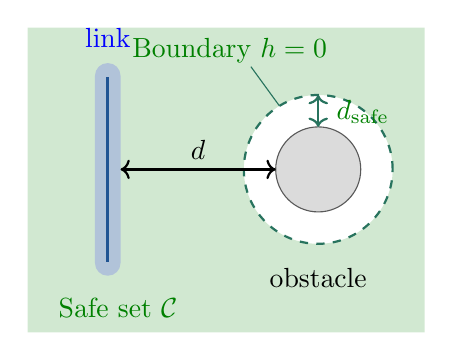
\begin{tikzpicture}[x=9mm,y=9mm]
        \path[use as bounding box] (-.3,-.65) rectangle (5.3,3.65);
        % Shade the safe side of the clearance boundary in this distance schematic.
        \fill[EmphasisGreen!18,even odd rule]
        (-.3,-.65) rectangle (5.3,3.65) (3.8,1.65) circle(1.05);
        % Surface distance: link capsule radius .18, obstacle radius .6.
        \fill[Accent!35,rounded corners=1.6mm](.65,.15)rectangle(1.01,3.15);
        \draw[line width=1pt,Accent](.83,.35)--(.83,2.95);
        \filldraw[fill=black!14,draw=black!65](3.8,1.65)circle(.6);
        \draw[dashed,Success,thick](3.8,1.65)circle(1.05);
        \draw[<->,thick](1.01,1.65)--node[above]{$d$}(3.2,1.65);
        \draw[<->,Success,thick](3.8,2.25)--(3.8,2.70);
        \node[text=EmphasisGreen,anchor=west]at(3.92,2.46){$d_{\mathrm{safe}}$};
        \node[text=EmphasisBlue]at(.83,3.5){link};
        \node at(3.8,.12){obstacle};
        \node[text=EmphasisGreen]at(2.55,3.32){Boundary $h=0$};
        \draw[Success](2.85,3.1)--(3.25,2.55);
        \node[text=EmphasisGreen,anchor=west]at(0,-.3){Safe set $\mathcal C$};
      \end{tikzpicture}
      \column{.49\textwidth}\raggedright
      \hspace*{5mm}%
      \begin{tabular}{@{}l@{}}
        \textcolor{EmphasisGreen}{\textbf{Safe set}}                         \\[1mm]
        {\color{EmphasisGreen}$\displaystyle\mathcal C=\{q\mid h(q)\geq0\}$} \\[4mm]
        \textbf{CBF constraint}                                              \\[1mm]
        $\displaystyle\dot h = \nabla_qh^\top u\geq-\gamma h,\quad\gamma>0$  \\[4mm]
        \textbf{Boundary condition}                                          \\[1mm]
        $\displaystyle h=0\quad\Rightarrow\quad\dot h\geq0$
      \end{tabular}
    \end{columns}
    \vfill
    $h>0$: motion toward obstacles allowed within the CBF constraint\par
    \vfill
  \end{slidebody}
\end{frame}

\begin{frame}[label=background-qp]{QP-Based Kinematic Control~\cite{ames2017cbf}}
  \framesubtitle{2.3 CLF-CBF QP}
  \begin{slidebody}
    \centering
    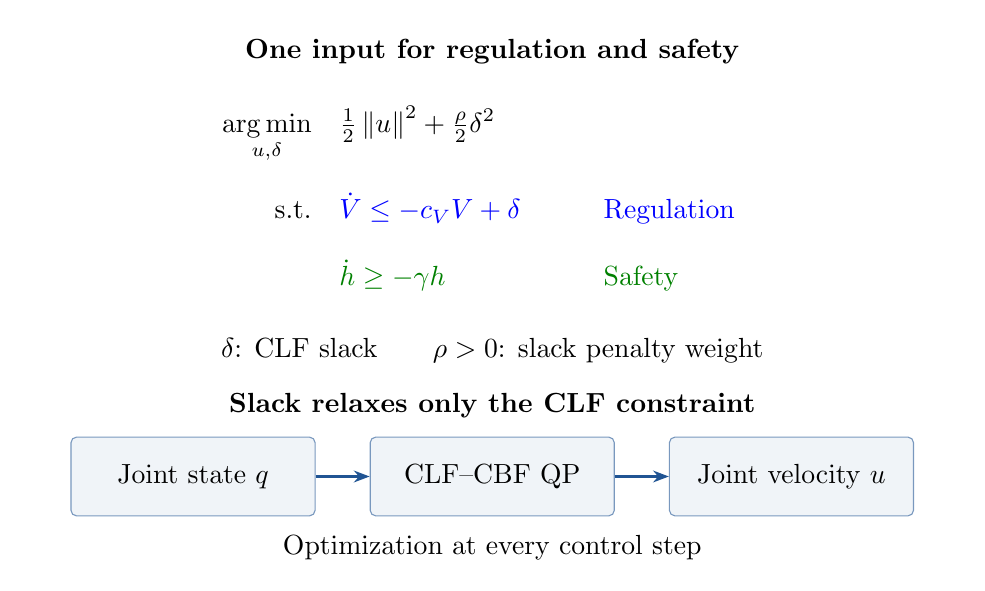
\begin{tikzpicture}[x=1mm,y=-1mm,
        copy/.style={inner sep=0pt,font=\normalsize,align=center}]
      \path[use as bounding box](0,-1)rectangle(118,67);
      \node[copy,font=\normalsize\bfseries] at(59,2){One input for regulation and safety};
      \node[copy] at(59,21){$\begin{aligned}
            \argmin_{u,\delta}\quad & \tfrac12\norm{u}^2+\tfrac{\rho}{2}\delta^2                                             \\[2.5mm]
            \text{s.t.}\quad
                                    & {\color{EmphasisBlue}\dot V\leq-c_VV+\delta}
                                    & \qquad                                       & {\color{EmphasisBlue}\text{Regulation}} \\[2.5mm]
                                    & {\color{EmphasisGreen}\dot h\geq-\gamma h}
                                    &                                              & {\color{EmphasisGreen}\text{Safety}}
          \end{aligned}$};
      \node[copy] at(59,40){$\delta$: CLF slack\qquad $\rho>0$: slack penalty weight};
      \node[copy,font=\normalsize\bfseries] at(59,47){Slack relaxes only the CLF constraint};
      \node[box,text width=25mm](state)at(21,56){Joint state $q$};
      \node[box,text width=25mm](qp)at(59,56){CLF--CBF QP};
      \node[box,text width=25mm](u)at(97,56){Joint velocity $u$};
      \draw[arr](state)--(qp);\draw[arr](qp)--(u);
      \node[copy] at(59,65){Optimization at every control step};
    \end{tikzpicture}
  \end{slidebody}
\end{frame}

\begin{frame}[label=literature]{Related Work: Challenges in Regulation}
  \framesubtitle{2.3.1 Local Minima and Deadlock in CLF-CBF QP}
  \begin{slidebody}
    \textbf{Common challenge: stalling away from the goal}\par\vspace{3mm}
    \begingroup
    \setlength{\tabcolsep}{2mm}
    \renewcommand{\arraystretch}{1.12}
    \begin{tabularx}{\linewidth}{@{}>{\raggedright\arraybackslash}p{25mm}
      >{\raggedright\arraybackslash}p{34mm}
      >{\raggedright\arraybackslash}X@{}}
      \textbf{Method} & \textbf{Design focus}                      & \textbf{How motion is guided} \\[1mm]
      \midrule
      Reis et al.~\cite{reis2021equilibria}
                      & CLF geometry
                      & Rotate the CLF to avoid gradient alignment                                 \\[3.5mm]
      Tan \& Dimarogonas~\cite{tan2024equilibria}
                      & Nominal input
                      & Center the QP on a CLF-compatible input                                    \\[3.5mm]
      Gon\c{c}alves et al.~\cite{goncalves2023circulation}
                      & Circulation constraint
                      & Induce tangential motion near obstacles
    \end{tabularx}
    \endgroup
    \vfill
    \begin{beamercolorbox}[sep=2mm,wd=\linewidth]{block body}
      \textcolor{EmphasisBlue}{\textbf{Research question}}\par\vspace{2mm}
      How can the manipulator's \textbf{kinematic structure}\\
      guide progress toward the goal?
    \end{beamercolorbox}
    \vspace{2mm}
  \end{slidebody}
\end{frame}

\begin{frame}[label=planar-direct]{A Naive Trial: Direct End-Effector Tracking}
  \framesubtitle{2.3.1 Local Minima and Deadlock in CLF-CBF QP}
  \begin{slidebody}
    \centering
    \textbf{Direct: end-effector (EE) regulation only}\par
    \vfill
    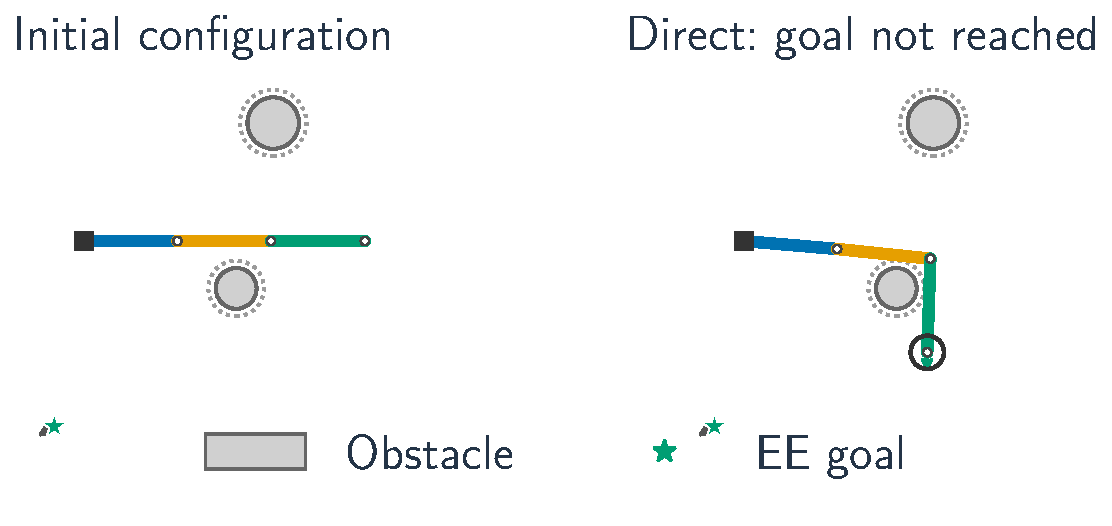
\includegraphics[width=\linewidth,height=55mm,keepaspectratio]{concept_planar_direct.pdf}\par
    \vfill
    $V=V_{\mathrm e}$: the final EE CLF from the start\par
    \vfill
  \end{slidebody}
\end{frame}

\defensepart{Planar}

\begin{frame}[label=human-inspiration]{Human-Inspired Intuition: Posture and Subgoals}
  \framesubtitle{1.2 Research Objectives}
  \begin{slidebody}
    \centering
    \begin{tikzpicture}[x=1mm,y=-1mm,
        copy/.style={font=\normalsize,inner sep=0pt,align=center}]
      \path[use as bounding box](0,-1)rectangle(118,67);
      \node[copy,anchor=north west,text width=64mm,align=left] at(0,0){%
        \textbf{Arm posture} shapes\\obstacle avoidance~\cite{menger2012posture}\\[3mm]
        \textbf{Subgoals} can organize reaching~\cite{lukic2014coordination}};
      \node[anchor=north east,inner sep=0pt] at(118,0){%
        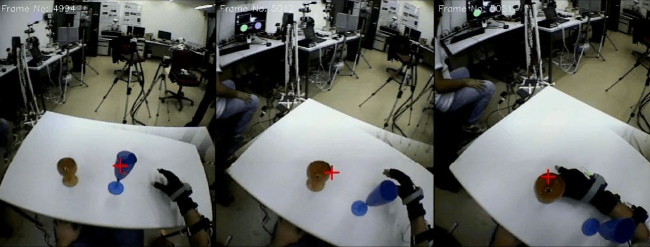
\includegraphics[width=50mm]{human_demonstration_lukic2014.png}};
      \node[copy,anchor=north,text width=50mm,font=\fontsize{7}{8.4}\selectfont] at(93,21){%
        Human demonstration: Lukic et al.~\cite{lukic2014coordination}};
      \node[copy,font=\normalsize\bfseries,text=EmphasisBlue] at(59,29){Design intuition: conceptual illustration};
      \foreach \shift/\a/\b/\caption in {14/-50/-30/Initial posture,53/70/30/During reaching,92/60/-15/Goal reached}{
          \begin{scope}[shift={(\shift,43)}]\begin{scope}[scale=.8]
              \fill[black!20](-3.685,3.685)rectangle(-.536,-4.02);
              \filldraw[fill=black!12,draw=black!50](11.725,0)rectangle(15.41,-4.355);
              \coordinate(S)at(0,0);
              \coordinate(E)at({10.05*cos(\a)},{-10.05*sin(\a)});
              \coordinate(H)at({10.05*cos(\a)+8.71*cos(\b)},{-10.05*sin(\a)-8.71*sin(\b)});
              \draw[line width=2.5pt,Accent](S)--(E);
              \draw[line width=2.5pt,Success](E)--(H);
              \fill[Accent](S)circle(2pt);\fill[black](E)circle(1.5pt);
              \draw[Success,fill=white,line width=1pt](H)circle(2pt);
              \node[star,star points=5,fill=Success,inner sep=2pt]at(13.4402,-6.4521){};
            \end{scope}\node[copy,text width=38mm]at(4.8,12){\caption};
          \end{scope}
        }
      \draw[arr](35,43)--(42,43);
      \draw[arr](74,43)--(81,43);
      \node[copy,fill=Soft,text width=114mm,minimum height=9mm,inner sep=2mm] at(59,64){\textbf{Our design:} IK-derived link targets $\longrightarrow$ EE goal};
    \end{tikzpicture}\par
  \end{slidebody}
\end{frame}

\begin{frame}[label=thesis-outline]{Chapter 3: Method Overview}
  \framesubtitle{3 A Sequential Approach to Collision-Free Kinematic Control}
  \begin{slidebody}
    \vfill
    \begin{tabularx}{\linewidth}{@{}l@{\hspace{5mm}}X@{}}
      \quad \textbf{3.1} & Problem Formulation                           \\[8mm]
      \quad \textbf{3.2} & Sequential Kinematic Control Framework        \\[8mm]
      \quad \textbf{3.3} & Application to the 3-DOF Planar Manipulator   \\[8mm]
      \quad \textbf{3.4} & Extension to the 7-DOF Spatial Manipulator    \\[8mm]
      \quad \textbf{3.5} & Learning-Based Selection of Two Link Subtasks
    \end{tabularx}
    \vfill
  \end{slidebody}
\end{frame}

\begin{frame}[label=planar-scene]{Proposed Method: Initial State, Goal, and Obstacles}
  \framesubtitle{3.2.1 Decomposition of Regulation Task}
  \begin{slidebody}
    \planarstage{progressive_planar_02_scene.pdf}{%
      \textbf{1 / 2: Task specification}\par\vspace{7mm}
      Initial state $q_0$\par\vspace{5mm}
      \textbf{EE regulation task $\regtask$}\\[1mm]
      Goal $(p_{\mathrm d},\psi_{\mathrm d})$\par\vspace{5mm}
      Obstacles $\mathcal O$}
  \end{slidebody}
\end{frame}

\begin{frame}[label=planar-setup]{Proposed Method: IK-Derived Link Subtasks}
  \framesubtitle{3.2.1 Decomposition of Regulation Task}
  \begin{slidebody}
    \planarstage{progressive_planar_03_ik.pdf}{%
      {\color{EmphasisBlue}\textbf{2 / 2: From IK to subtasks}}\par\vspace{4mm}
      \textbf{Selected IK posture $q^*$}\\[1mm]
      Dashed: whole-arm posture\par\vspace{2mm}
      $\Downarrow$\par\vspace{2mm}
      \textbf{Link subtask targets}\\[1mm]
      $p_i^*=p_i(q^*)$\par\vspace{2mm}
      \textbf{Subtasks $\subtask{s}$} ($s=1,2,3$)\par\vspace{2mm}
      \textbf{Sequential:} $\subtask{1}\to\subtask{2}\to\subtask{3}$\par\vspace{2mm}
      Final subtask: $\subtask{3}=\regtask$\par\vspace{2mm}
      Link order: $\mathcal S=(1,2,3)$}
  \end{slidebody}
\end{frame}

\begin{frame}[label=planar-sequential]{Sequential: Link 1 Subtask}
  \framesubtitle{3.2.2 CLF-CBF QP-Based Kinematic Control}
  \begin{slidebody}
    \planarstage{progressive_planar_04_link1.pdf}{\taskqp{1}{EmphasisBlue}{c_1}}
  \end{slidebody}
\end{frame}

\begin{frame}[label=planar-link2]{Sequential: Link 2 Subtask}
  \framesubtitle{3.2.2 CLF-CBF QP-Based Kinematic Control}
  \begin{slidebody}
    \planarstage{progressive_planar_05_link2.pdf}{\taskqp{2}{EmphasisOrange}{c_2}}
  \end{slidebody}
\end{frame}

\begin{frame}[label=planar-ee]{Sequential: End-Effector Subtask}
  \framesubtitle{3.2.2 CLF-CBF QP-Based Kinematic Control}
  \begin{slidebody}
    \planarstage{progressive_planar_06_ee.pdf}{\taskqp{3}{EmphasisGreen}{c_3}}
  \end{slidebody}
\end{frame}

\begin{frame}[label=planar-clf]{Planar CLFs: One QP and One CLF at Each Stage}
  \framesubtitle{3.3.2 Intermediate Position Tasks and Final Pose Task}
  \begin{slidebody}
    \centering $\subtask{1}\to\subtask{2}\to\subtask{3}=\regtask$\par\vspace{1mm}
    \begin{tikzpicture}[x=\linewidth,y=1mm,
        formula/.style={font=\normalsize,inner sep=0pt}]
      \path[use as bounding box](0,-56.5)rectangle(1,5);
      \node[font=\normalsize\bfseries,text=EmphasisBlue] (q1) at (.16,0){$\mathrm{QP}_1$};
      \node[font=\normalsize\bfseries,text=EmphasisOrange] (q2) at (.50,0){$\mathrm{QP}_2$};
      \node[font=\normalsize\bfseries,text=EmphasisGreen] (qe) at (.84,0){$\mathrm{QP}_{3}$};
      \draw[arr](q1.east)--node[midway,above=1mm,font=\normalsize]{Subtask transition}(q2.west);
      \draw[arr](q2.east)--node[midway,above=1mm,font=\normalsize]{Subtask transition}(qe.west);
      \node[anchor=north,inner sep=0pt] at(.16,-2.5){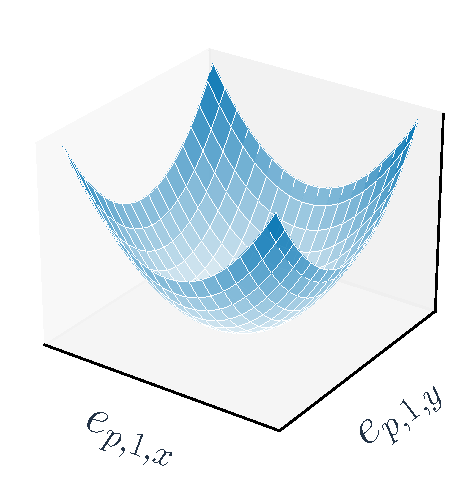
\includegraphics[width=.2944\linewidth,height=24mm,keepaspectratio]{concept_clf_1.pdf}};
      \node[anchor=north,inner sep=0pt] at(.50,-2.5){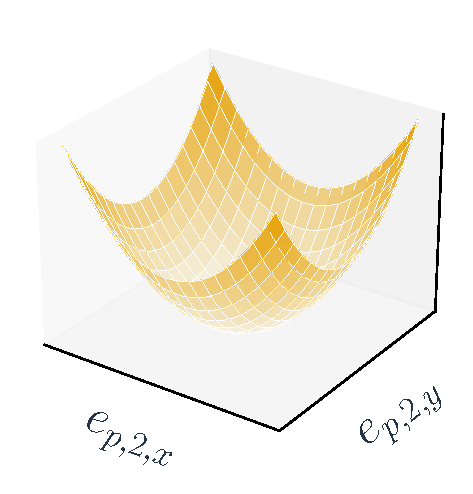
\includegraphics[width=.2944\linewidth,height=24mm,keepaspectratio]{concept_clf_2.pdf}};
      \node[anchor=north,inner sep=0pt] at(.84,-2.5){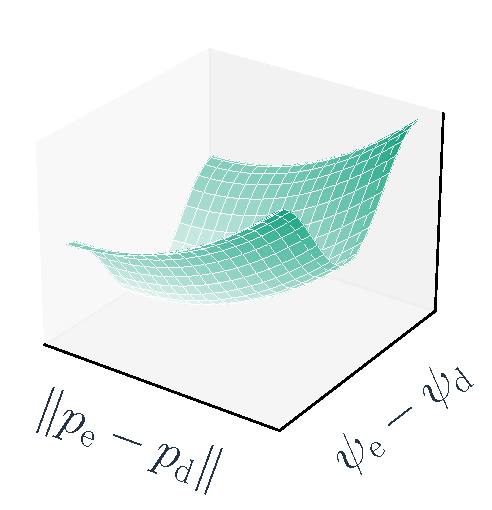
\includegraphics[width=.2944\linewidth,height=24mm,keepaspectratio]{concept_clf_ee.pdf}};
      \node[formula] at(.16,-30.5){$V_1=\tfrac12\norm{e_{\mathrm p,1}}^2$};
      \node[formula] at(.50,-30.5){$V_2=\tfrac12\norm{e_{\mathrm p,2}}^2$};
      \node[formula] at(.84,-30.5){$V_3=V_{\mathrm ee}$: position + yaw};
      \node[formula] at(.16,-39){\colorbox{Accent!12}{\strut$\dot V_1\leq-c_1V_1+\delta$}};
      \node[formula] at(.50,-39){\colorbox{orange!12}{\strut$\dot V_2\leq-c_2V_2+\delta$}};
      \node[formula] at(.84,-39){\colorbox{Success!12}{\strut$\dot V_3\leq-c_3V_3+\delta$}};
      \node[formula] at(.50,-47.5){$V_{\rm ee}=\tfrac12\norm{p_{\mathrm e}-p_{\mathrm d}}^2+\tfrac{w_{\mathrm o}}2[1-\cos(\psi_{\mathrm ee}-\psi_{\mathrm d})],\quad w_{\mathrm o}>0$};
      \node[formula] at(.50,-54.5){Unchanged QP objective, CBFs, and input limits};
    \end{tikzpicture}\par\vfill
  \end{slidebody}
\end{frame}

\begin{frame}[label=algorithm-overview]{Overall Sequential Control Framework}
  \framesubtitle{3.2 Sequential Kinematic Control Framework}
  \begin{slidebody}
    \centering
    \sequentialframework\par\vfill
  \end{slidebody}
\end{frame}

\begin{frame}[label=planar-results]{Planar Results: Direct 72.00\% / Sequential 84.33\%}
  \framesubtitle{4.1 System 1: 3-DOF Planar Model}
  \begin{slidebody}
    \centering
    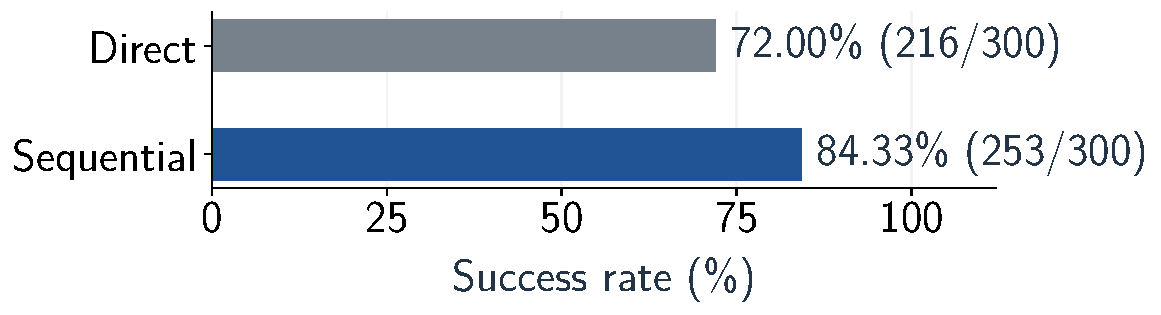
\includegraphics[width=.94\linewidth,height=38mm,keepaspectratio]{planar_success.pdf}\par
    \vfill
    \begin{columns}[T,onlytextwidth]
      \column{.48\textwidth}
      \textbf{300 IK episodes}
      \begin{itemize}\setlength{\itemsep}{1mm}
        \item 1 m per link; 2 obstacles
        \item Initial $q_0=(0,0,0)$
        \item Time limit $T_{\mathrm d}=35$ s
      \end{itemize}
      \column{.46\textwidth}
      \textbf{Success on the same 300 episodes}\par\vspace{1mm}
      \begin{tabular}{lr}\toprule
        Sequential only  & 47          \\[1mm]
        Direct only      & 10          \\[1mm]
        Net success gain & \textbf{37} \\\bottomrule
      \end{tabular}
    \end{columns}
    \vfill
    \centering Success: EE goal reached safely within 35 s\par

  \end{slidebody}
\end{frame}

\begin{frame}[label=planar-why]{Resolving Deadlock through Subtask Transition}
  \framesubtitle{4.1.2 Paired Outcomes and an Illustrative Trajectory}
  \begin{slidebody}
    \takeaway{Link subtasks allow temporary increases in EE error}
    \vspace{1mm}
    \centering
    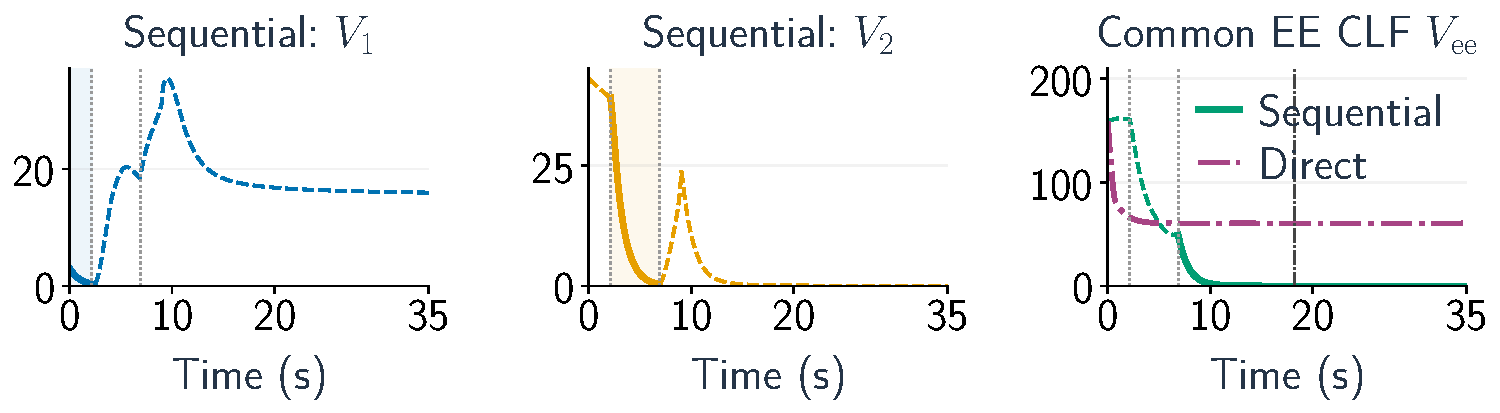
\includegraphics[width=\linewidth,height=35mm,keepaspectratio]{case030_clf_time.pdf}\par\vspace{1mm}
    {\normalsize Solid/shaded: active / dashed: inactive / purple: Direct}
    \vfill
    \begin{itemize}\setlength{\itemsep}{4mm}
      \item Direct: final-goal tracking can settle at a non-goal equilibrium
      \item Sequential: a new subtask changes the feasible tracking direction
    \end{itemize}

  \end{slidebody}
\end{frame}

\defensepart{Spatial}

\begin{frame}[label=panda-extension]{Extension to a 7-DOF Spatial Manipulator}
  \framesubtitle{3.4 Extension to the 7-DOF Spatial Manipulator}
  \begin{slidebody}
    \begin{columns}[c,onlytextwidth]
      \column{.45\textwidth}\centering
      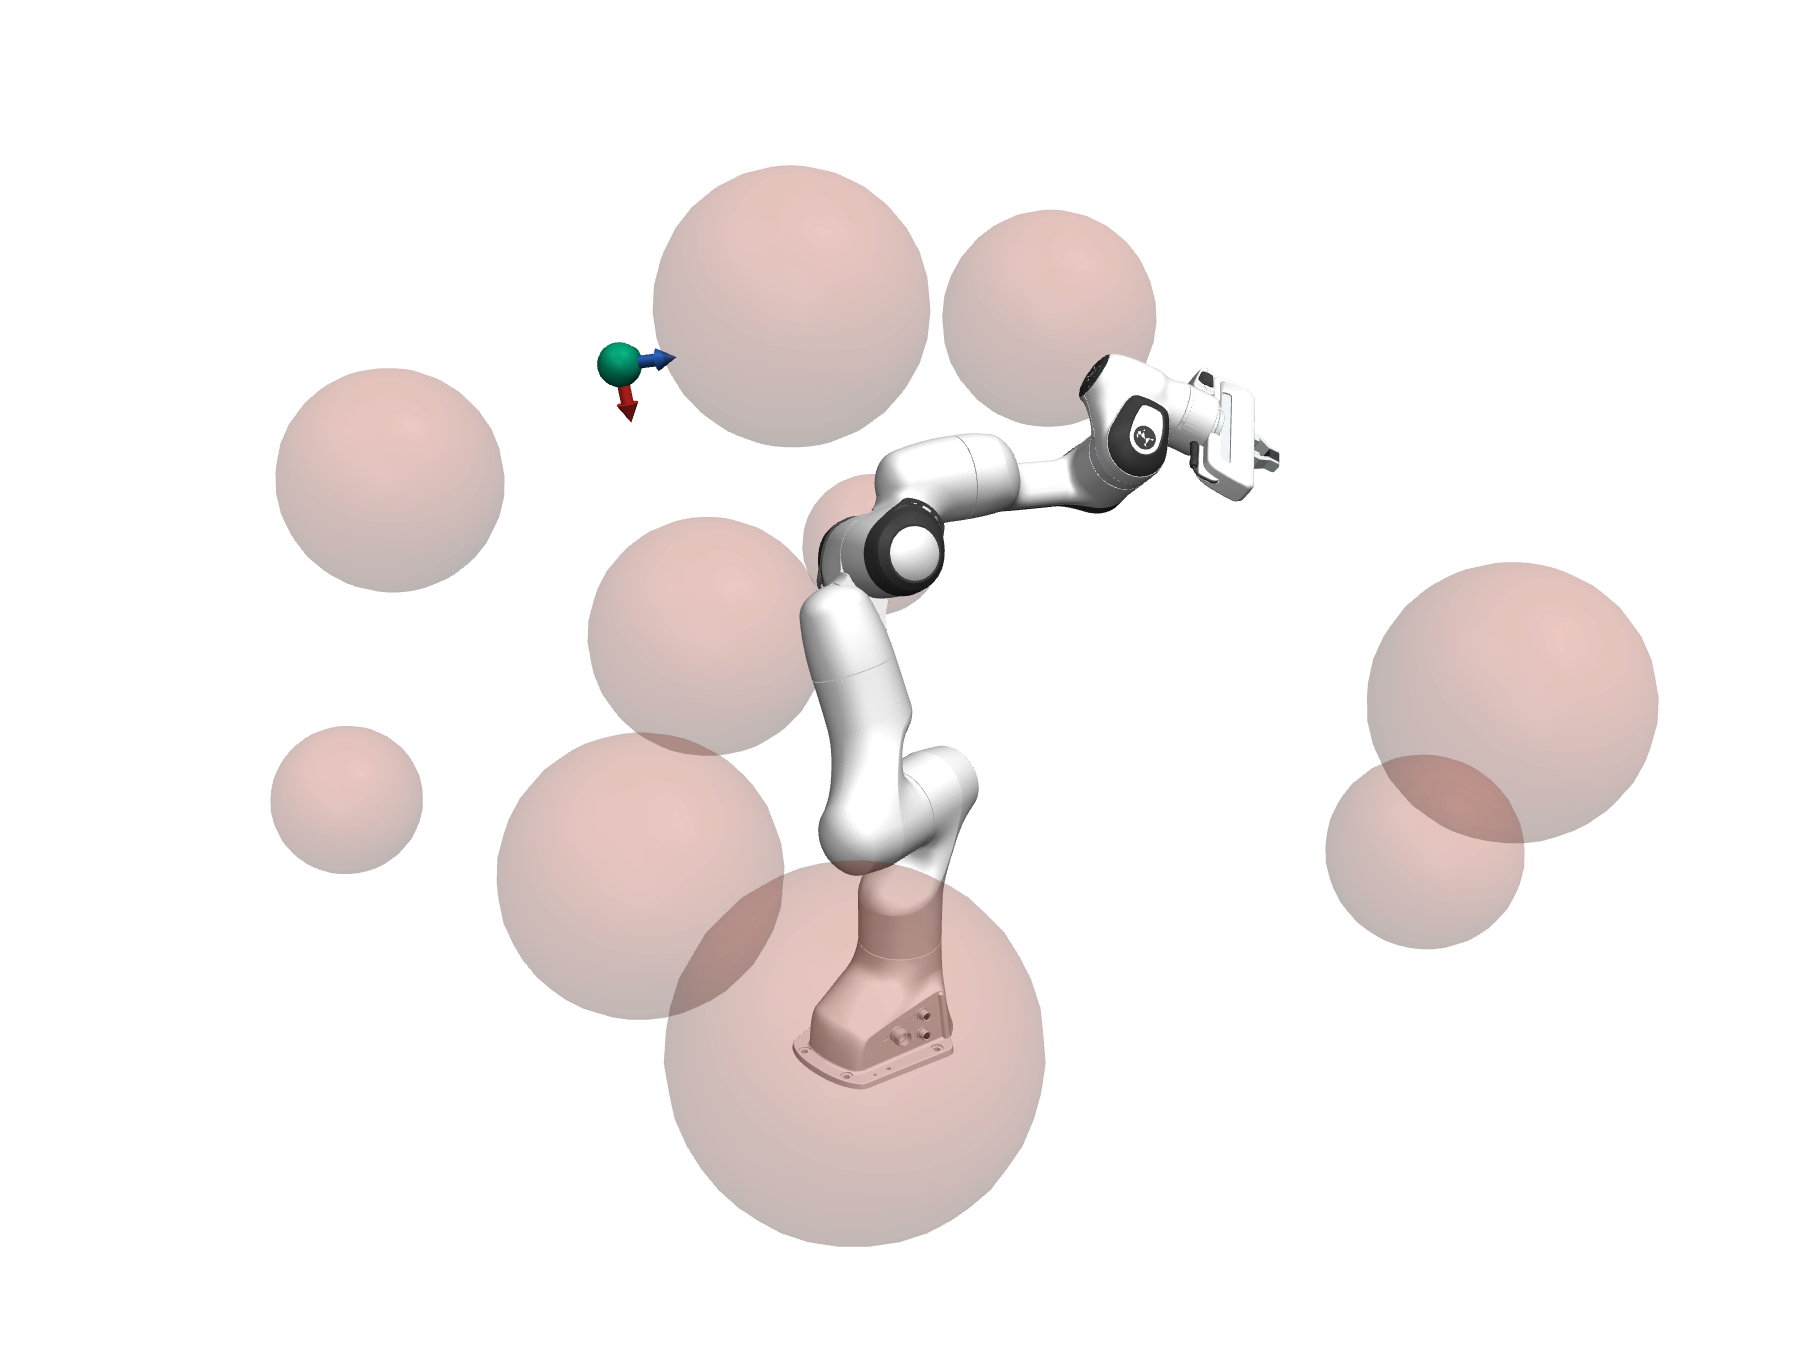
\includegraphics[width=\linewidth,height=33mm,keepaspectratio]{panda_mujoco.png}\par\vspace{1mm}
      MuJoCo: initial state and goal
      \column{.51\textwidth}
      \textbf{Same sequential framework}\par\vspace{3mm}
      \begin{itemize}\setlength{\itemsep}{3mm}
        \item Collision-free IK among redundant solutions
        \item Self-collision avoidance for complex link shapes
      \end{itemize}
    \end{columns}\par\vfill
    \begin{tabularx}{\linewidth}{@{}lXX@{}}\toprule
      Component       & Planar manipulator & Spatial Manipulator     \\\midrule
      Configuration   & $q\in\mathbb R^3$  & $q\in\mathbb R^7$       \\[2mm]
      Task error      & Position / yaw     & Position / quaternion   \\[2mm]
      Collision model & Capsule distances  & Capsule + RDF distances \\\bottomrule
    \end{tabularx}\par\vfill
  \end{slidebody}
\end{frame}

\begin{frame}[label=panda-rdf]{Self-Collision CBFs from Robot Distance Field~\cite{li2024rdf}}
  \framesubtitle{3.4.3 RDF-Based Construction of CBF}
  \begin{slidebody}
    \begin{columns}[c,onlytextwidth]
      \column{.48\textwidth}\centering
      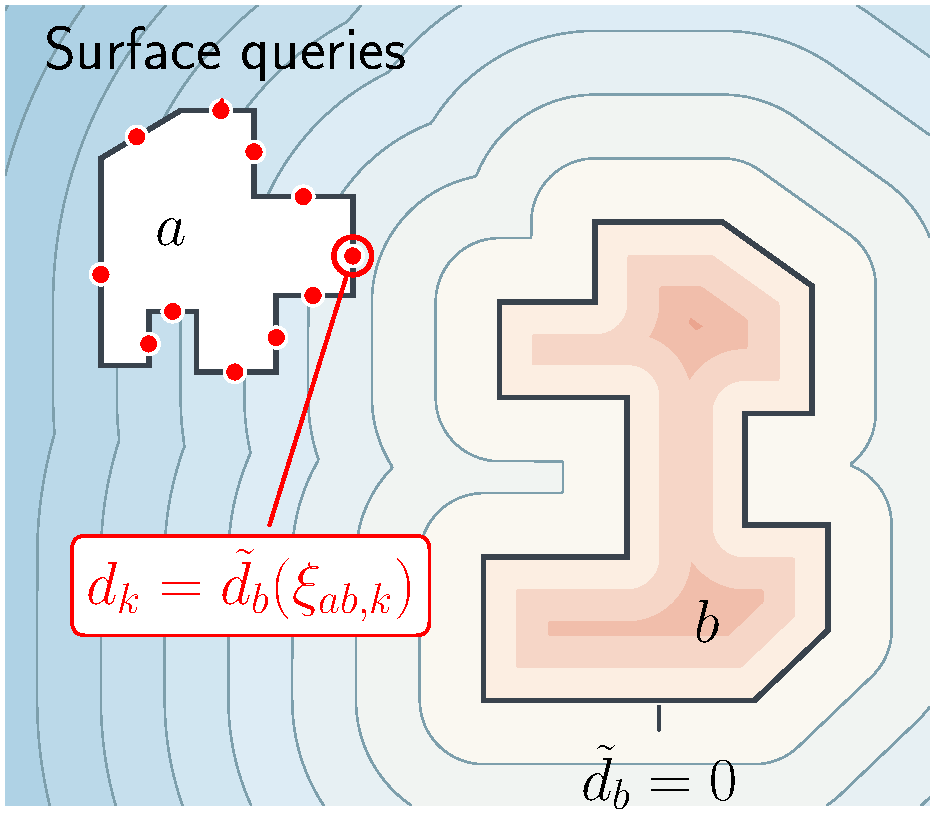
\includegraphics[width=\linewidth,height=51mm,keepaspectratio]{rdf_complex_query_field.pdf}\par\vspace{1mm}
      2D query illustration
      \column{.46\textwidth}\raggedright
      $a$: source link; $b$: target link\par\vspace{3mm}
      \begin{tabular}{@{}l@{}}
        \textbf{1. Transform queries}                       \\[1.5mm]
        $\displaystyle\xi_{ab,k}=R_b^\top(x_{a,k}-p_b)$     \\[4mm]
        \textbf{2. Evaluate $b$'s RDF}                      \\[1.5mm]
        $\displaystyle d_k=\tilde d_b(\xi_{ab,k})$          \\[4mm]
        \textbf{3. Construct $h_{ab}(q)$}                   \\[1.5mm]
        $\displaystyle D_{ab}=\operatorname{softmin}_k d_k$ \\[1.5mm]
        $\displaystyle h_{ab}=D_{ab}-m_{\mathrm{phys}}-m_{\mathrm{err}}$
      \end{tabular}
    \end{columns}\par\vfill
    \textbf{CBF gradient:} account for both links' motion\par\vspace{2mm}
    \centering $\nabla_qh_{ab}^{\top}u\geq-\gamma h_{ab}$\par
  \end{slidebody}
\end{frame}

\begin{frame}[label=panda-ik]{Spatial IK: Target Search with Null-Space Updates}
  \framesubtitle{3.4.1 Multi-Start IK with a Safety-Aware Null-Space Update}
  \begin{slidebody}
    \setlength{\abovedisplayskip}{3pt}
    \setlength{\belowdisplayskip}{3pt}

    \begin{block}{EE-error correction + clearance improvement~\cite{siciliano2009robotics}}
      \[v_{\mathrm{IK}}=
        \underbrace{J_\lambda^\# k_pe_{\mathrm{IK}}}_{\text{EE-error correction}}
        +\underbrace{(I-J^\dagger J)k_h\nabla H_\tau}_{v_h:\ \text{null-space term}}\]
    \end{block}
    \vfill
    \[H_\tau=-\tau\log\sum_r e^{-h_r^{\mathrm{IK}}/\tau}\]
    \[Jv_h=0,\qquad \nabla H_\tau^\top v_h\geq0\]
    \centering Clearance improvement without changing the EE twist\par
    \vfill
    \begin{enumerate}\setlength{\itemsep}{3mm}
      \item Capsule-based search from multiple initial guesses
      \item Acceptance of $q^*$ after goal, joint-limit, and RDF collision checks
    \end{enumerate}

  \end{slidebody}
\end{frame}

\begin{frame}[label=panda-clf]{Spatial CLFs: Position and Orientation}
  \framesubtitle{3.4.2 All-Link Sequence and Spatial Pose Tasks}
  \begin{slidebody}

    \begin{tabularx}{\linewidth}{@{}lXX@{}}\toprule
      Model               & Link subtasks          & Final EE subtask       \\\midrule
      Planar              & position               & position + yaw         \\[3mm]
      Spatial Manipulator & position + orientation & position + orientation \\\bottomrule
    \end{tabularx}
    \vfill
    \begin{block}{Identical CLF form for link and EE subtasks}
      \centering Link subtask $\subtask{s}$: $i=i_s$, $s=1,\ldots,L$
      \[V_i=\tfrac12\norm{p_i-p_i^*}^2+
        \tfrac{w_R}{2}\norm{\epsilon_i}^2\]
      \[[\eta_i,\epsilon_i^\top]^\top=Q_i^*Q_i^{-1}\]
    \end{block}
    \vfill
    \centering
    $\epsilon_i$: vector part of the relative unit quaternion\par
    \vspace*{6mm}
  \end{slidebody}
\end{frame}

\begin{frame}[label=all-links]{All-link Sequential: Spatial Manipulator Results}
  \framesubtitle{4.2.2 Effect of All-Link Sequential Control}
  \begin{slidebody}

    \begin{block}{All-link Sequential: seven link subtasks, then the EE subtask}
      \centering
      $\underbrace{\subtask{1}\to\cdots\to\subtask{7}}_{L=7\ \text{link subtasks}}\to\subtask{8}=\regtask$
    \end{block}
    \vfill
    \centering
    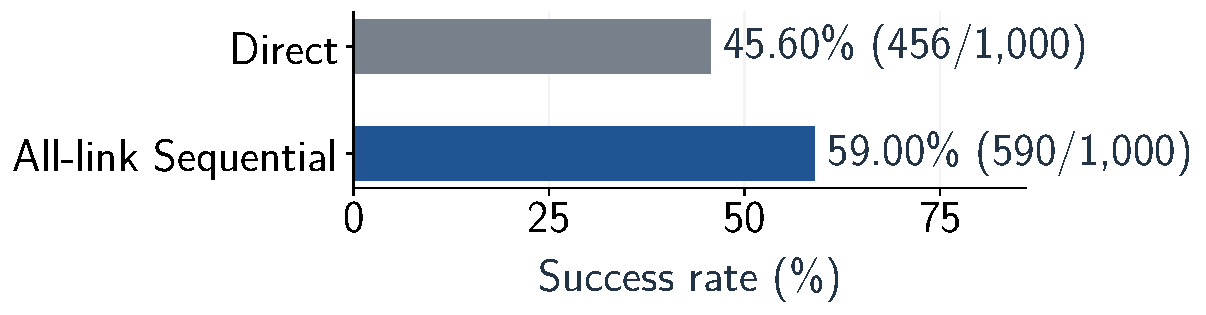
\includegraphics[width=.96\linewidth,height=38mm,keepaspectratio]{panda_all_links.pdf}\par
    \vfill
    \textbf{Validation:} 1,000 IK episodes / 10 obstacles / 120 s\par
    \vspace{2mm}Success: EE goal reached safely within 120 s\par

  \end{slidebody}
\end{frame}

\begin{frame}[label=time-cost]{The Completion-Time Cost of All-link Sequential Control}
  \framesubtitle{4.2.2 Effect of All-Link Sequential Control}
  \begin{slidebody}
    \takeaway{Longer completion time for All-link Sequential}

    \centering
    \textbf{Validation: 330 episodes with success in both methods}\par
    \vfill
    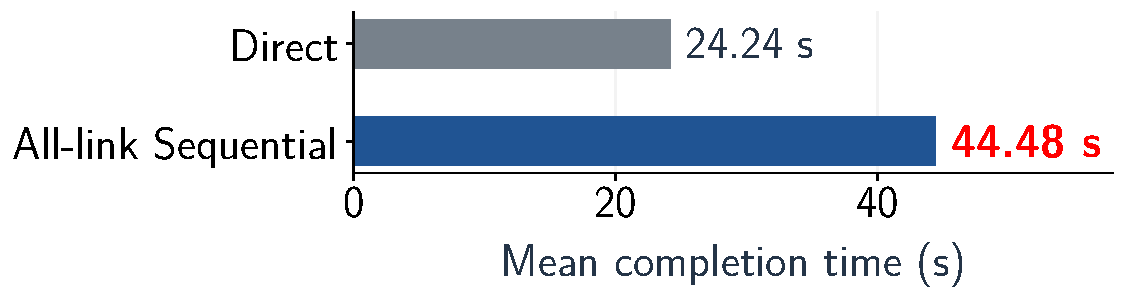
\includegraphics[width=.95\linewidth,height=43mm,keepaspectratio]{story_time_cost.pdf}\par
    \vfill
    \begin{itemize}\setlength{\itemsep}{2.5mm}
      \item Mean completion time: 24.24 s $\to$ \textcolor{EmphasisRed}{\textbf{44.48 s}}
      \item Seven link subtasks before the EE subtask
    \end{itemize}

  \end{slidebody}
\end{frame}

\begin{frame}[label=two-links]{Reduction to Two Link Subtasks}
  \framesubtitle{4.2.3 Two-Link Reduction: Completion Time and Success}
  \begin{slidebody}
    \takeaway{Select two link subtasks before the EE subtask}
    \begin{block}{Link subtasks: 7 $\to$ 2 / total subtasks: 8 $\to$ 3}
      \centering
      $\Omega=\{(a,b):2\leq a<b\leq6\}$, 10 candidate pairs\\[2mm]
      $\underbrace{\subtask{1}}_{\text{link }a}\to\underbrace{\subtask{2}}_{\text{link }b}\to\subtask{3}=\regtask$
    \end{block}
    \vfill
    \begin{tabularx}{\linewidth}{@{}Xrr@{}}\toprule
      Validation          & Success rate                                          & Mean time (s) \\\midrule
      All-link Sequential & 59.00\%                                               & 46.99         \\[2mm]
      10-pair mean        & 54.73\%                                               & 35.05         \\[2mm]
      Change              & \textcolor{EmphasisRed}{\textbf{\boldmath$-4.27$\%p}}
                          & \textcolor{EmphasisRed}{\textbf{\boldmath$-25.41$\%}}                 \\\bottomrule
    \end{tabularx}
    \vfill
    Time: 4,545 common-success episode--pair outcomes\par
  \end{slidebody}
\end{frame}

\defensepart{Learning}

\begin{frame}[label=oracle]{Link-Pair Selection: A Potential Upper Bound near 80\%}
  \framesubtitle{4.2.3 Two-Link Reduction: Completion Time and Success}
  \begin{slidebody}
    \takeaway{Oracle 82.00\%: post-hoc bound from all 10 candidate rollouts}

    \centering
    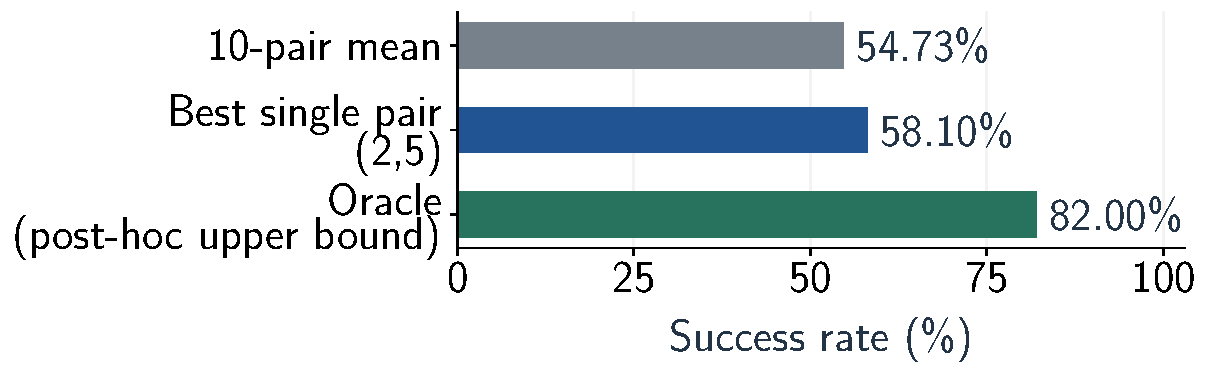
\includegraphics[width=\linewidth,height=42mm,keepaspectratio]{story_oracle_average.pdf}\par
    \vfill
    \begin{itemize}\setlength{\itemsep}{3mm}
      \item Validation: a successful pair in 820/1,000 episodes
      \item Potential gain from selecting a different pair for each episode
    \end{itemize}

  \end{slidebody}
\end{frame}

\begin{frame}[label=selector-training]{Training Labels and Losses}
  \framesubtitle{3.5.4 Training Objective and Sequence Selection}
  \begin{slidebody}
    \begin{block}{Episode labels $y_k$: 1 = success, 0 = failure}
      \centering
      \setlength{\tabcolsep}{3pt}
      \begin{tabular}{cccccccccc}
        $(2,3)$                               & $(2,4)$ & $(2,5)$ & $(2,6)$                               & $(3,4)$ & $(3,5)$ & $(3,6)$ & $(4,5)$ & $(4,6)$ & $(5,6)$ \\
        \textcolor{EmphasisGreen}{\textbf{1}} & 0       & 0       & \textcolor{EmphasisGreen}{\textbf{1}} & 0       & 0       & 0       & 0       & 0       & 0
      \end{tabular}
    \end{block}
    \vfill
    {\color{EmphasisBlue}\textbf{Binary Cross Entropy: predict each pair's success}}\par
    \vspace{2mm}
    {\centering\(
      \ell_{\mathrm{BCE}}=-\frac1{10}\sum_{k=1}^{10}
      \bigl[y_k\log\hat p_k+(1-y_k)\log(1-\hat p_k)\bigr]
      \)\par\vspace{1mm}
      Model logits $a_k$\quad $\hat p_k=\sigma(a_k)$\par}
    \vfill
    {\color{EmphasisBlue}\textbf{Selection: put weight on successful pairs}}\par
    \vspace{2mm}
    {\centering\(
    \ell_{\mathrm{sel}}=
    \begin{cases}
      -\log\sum_{k:y_k=1}\omega_k, & \text{any successful pair}, \\[1mm]
      0,                           & \text{all pairs fail},
    \end{cases}
    \qquad \omega_k=\dfrac{e^{a_k}}{\sum_{j=1}^{10}e^{a_j}}
    \)\par}
    \vfill
    {\centering\(\mathcal L=\frac1{N_{\mathrm{tr}}}\sum_{n=1}^{N_{\mathrm{tr}}}
    \bigl(\ell_{\mathrm{BCE},n}+\lambda_{\mathrm{sel}}\ell_{\mathrm{sel},n}\bigr),\quad\lambda_{\mathrm{sel}}=3\)\par}
    \vspace{2mm}
    \centering\normalsize Train 21,423 / Validation 1,000 / Test 1,000 episodes
  \end{slidebody}
\end{frame}

\begin{frame}[label=selector-features]{Learned Selection (1/2): Predicting Success Scores}
  \framesubtitle{3.5.3 Network Architecture}
  \begin{slidebody}
    \takeaway{Before execution: score each candidate link pair}
    \centering
    \selectorfigure{1}\par\vfill

  \end{slidebody}
\end{frame}

\begin{frame}[label=selector-model]{Learned Selection (2/2): From Subtasks to QP}
  \framesubtitle{3.5.3 Network Architecture}
  \begin{slidebody}
    \takeaway{Select once before execution; solve the QP at every control step}
    \centering
    \selectorfigure{2}\par

  \end{slidebody}
\end{frame}

\defensepart{Results}

\begin{frame}[label=test-success]{Test Results: Goal-Reaching Success Rates}
  \framesubtitle{4.2.5 Recovery Through Learned Link Selection}
  \begin{slidebody}
    \centering
    \textbf{Test:} 1,000 IK episodes / identical success criteria\par\vspace{1mm}
    10-pair mean: average success across the candidate pairs\par\vfill
    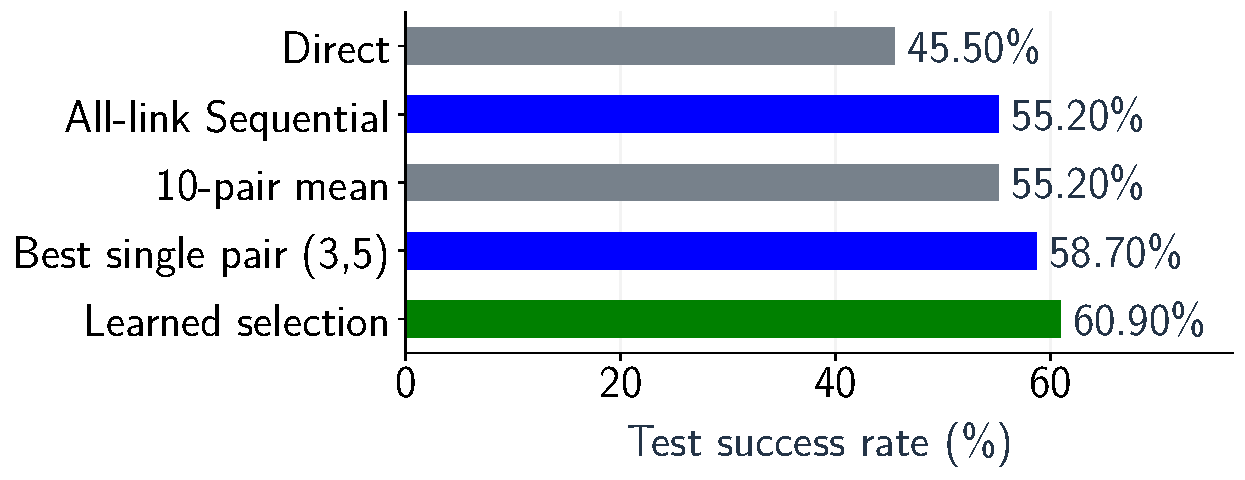
\includegraphics[width=\linewidth,height=44mm,keepaspectratio]{test_success_pair_mean.pdf}\par
    \vfill
    \begin{block}{Learned selection $-$ 10-pair mean: +5.70 pp}
      Paired 95\% confidence interval (CI): $[3.74,7.65]$\,pp
    \end{block}
  \end{slidebody}
\end{frame}

\begin{frame}[label=test-time]{Shorter Completion Time with Fewer Subtasks}
  \framesubtitle{4.2.3 Two-Link Reduction: Completion Time and Success}
  \begin{slidebody}
    \takeaway{Stage reduction retains the completion-time benefit}

    \centering
    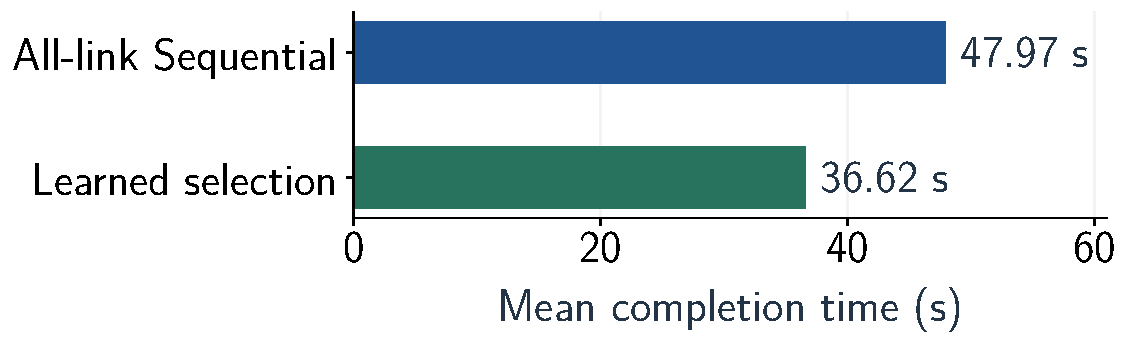
\includegraphics[width=.95\linewidth,height=43mm,keepaspectratio]{paired_time_test_all_links.pdf}\par\vfill
    \textbf{467 Test episodes with success in both methods}\par\vspace{3mm}
    Mean completion time: $47.97\to36.62$ s\par\vspace{2mm}
    \textbf{11.35 s shorter with two link subtasks}
  \end{slidebody}
\end{frame}

\begin{frame}[label=learning-why]{Why Selection Matters: Only One Pair Succeeds}
  \framesubtitle{4.2.5 Recovery Through Learned Link Selection}
  \begin{slidebody}
    \centering
    \textbf{Common initial state and each method's final configuration}\par
    \vfill
    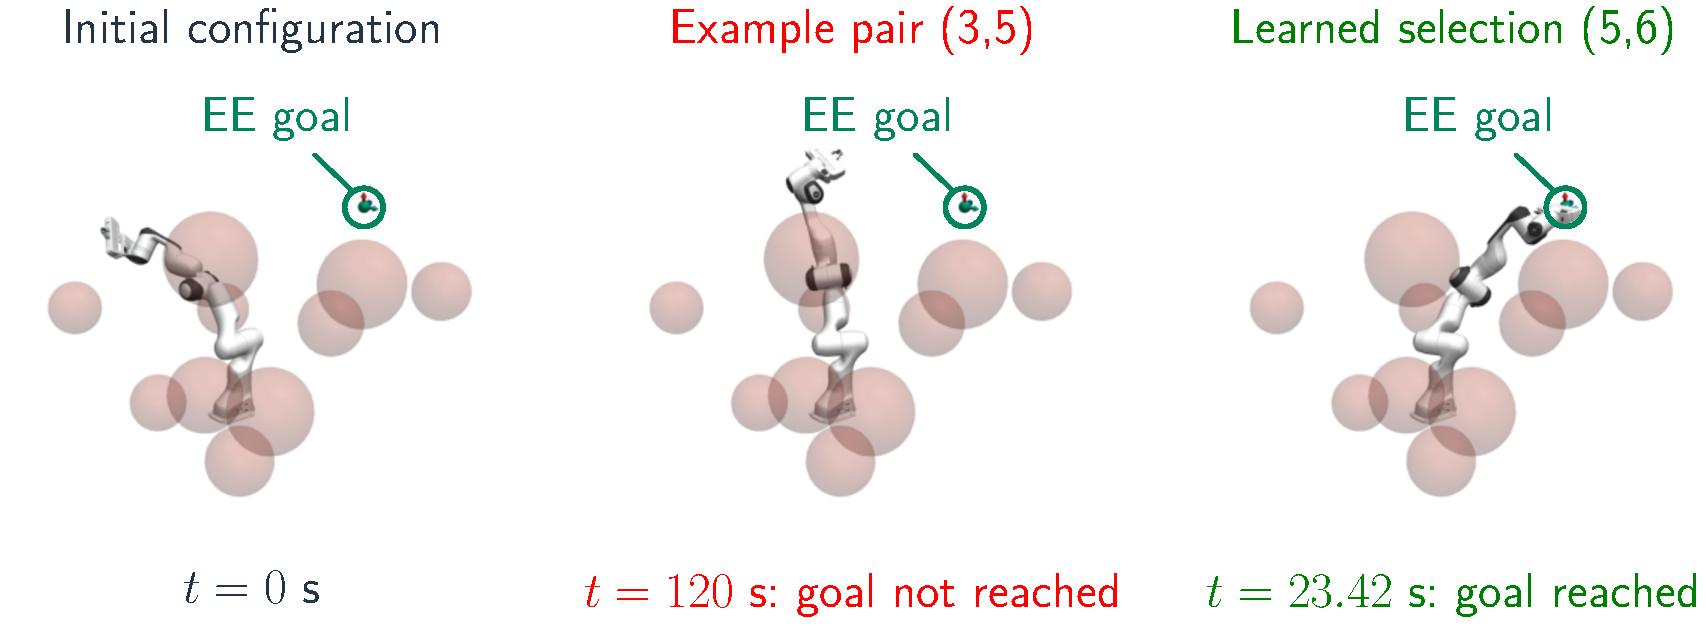
\includegraphics[width=\linewidth,height=49mm,keepaspectratio]{recovery_comparison.pdf}\par
    \vfill
    \begin{itemize}\setlength{\itemsep}{2mm}
      \item Example pair $(3,5)$: stopped at link 3 / selected $(5,6)$: EE goal reached
      \item Only $(5,6)$ succeeds among the 10 candidate pairs in this episode
    \end{itemize}

  \end{slidebody}
\end{frame}

\begin{frame}[label=conclusion]{Conclusions: Safe Control and Learned Sequencing}
  \framesubtitle{5 Conclusion}
  \begin{slidebody}

    \begin{enumerate}\setlength{\itemsep}{5mm}
      \item \textbf{IK-based subtask construction}\\[1mm]
            Higher observed success rates than Direct on Planar and Spatial Manipulator
      \item \textbf{Stage reduction to two link subtasks}\\[1mm]
            Shorter completion times than All-link Sequential
      \item \textbf{Learned link-pair selection for each episode}\\[1mm]
            Versus 10-pair mean: +5.70\,pp / 95\% CI $[3.74,7.65]$\,pp
    \end{enumerate}
    \vfill
  \end{slidebody}
\end{frame}

\begin{frame}[label=future-work]{Future Work: Experiments and Sequencing}
  \framesubtitle{4.2.6 Interpretation and Limitations}
  \begin{slidebody}
    \vfill
    \begin{enumerate}\setlength{\itemsep}{10mm}
      \item \textbf{Physical-robot experiments}
            \begin{itemize}\normalsize\setlength{\itemsep}{3mm}
              \item Closed-loop control on the physical robot
              \item Success rate, minimum margin, and completion time
            \end{itemize}
      \item \textbf{Neural-network-based sequencing improvements}
            \begin{itemize}\normalsize\setlength{\itemsep}{3mm}
              \item Relative-obstacle spatial features and network architecture
              \item Link subtask selection without a fixed count
            \end{itemize}
    \end{enumerate}
    \vfill
  \end{slidebody}
\end{frame}

\begin{frame}[c,label=questions]{}
  \centering
  {\color{Accent}\fontsize{28}{34}\selectfont\bfseries Thank you}\par
\end{frame}

\appendix

\begin{frame}{Appendix Contents}
  \hypertarget{appendix-contents}{}
  \begin{slidebody}
    \begin{columns}[t,onlytextwidth]
      \column{.48\textwidth}
      \begin{minipage}[t][67mm][s]{\linewidth}
        \begin{block}{\strut Control and geometry}
          \appendixentry{3}{Spatial IK safety term}
          \appendixentry{4}{RDF barrier derivatives}
          \appendixentry{12}{Common CLF--CBF QP}
          \appendixentry{13}{Control architecture}
        \end{block}
        \vfill
        \begin{block}{\strut Tasks and foundations}
          \appendixentry{5}{Stage-transition rules}
          \appendixentry{9}{Safe-set invariance}
          \appendixentry{11}{Goal criteria}
          \appendixentry{7}{References}
          \appendixentry{17}{Related-work assumptions}
        \end{block}
      \end{minipage}
      \column{.48\textwidth}
      \begin{minipage}[t][67mm][s]{\linewidth}
        \begin{block}{\strut Learning and evaluation}
          \appendixentry{2}{Validation success by pair}
          \appendixentry{6}{Paired test comparisons}
          \appendixentry{8}{Training and model selection}
          \appendixentry{14}{Evidence and limitations}
        \end{block}
        \vfill
        \begin{block}{\strut Episode diagnostics}
          \appendixentry{1}{Planar episode 11}
          \appendixentry{10}{Planar episode 30}
          \appendixentry{15}{Episode-wise selection gain}
          \appendixentry{16}{Boundary stagnation}
        \end{block}
      \end{minipage}
    \end{columns}
  \end{slidebody}
\end{frame}

\begin{frame}{A1. Full Diagnostics for Planar Episode 11}
  \hypertarget{appendix-a1}{}
  \framesubtitle{4.1 System 1: 3-DOF Planar Model}
  \begin{slidebody}
    \centering
    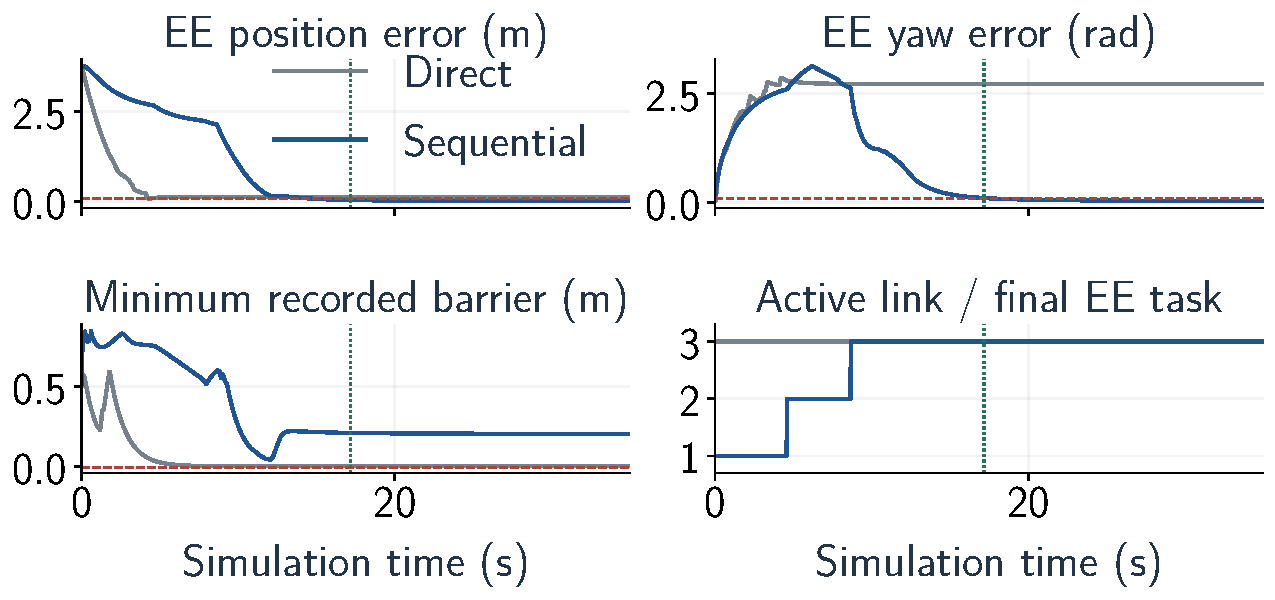
\includegraphics[width=.98\linewidth,height=54mm,keepaspectratio]{planar_trace.pdf}
    \vfill
    \begin{itemize}\normalsize
      \item Position, yaw, minimum barrier, and active link
      \item Red dashed: evaluation tolerance / green: first success at 17.176 s
    \end{itemize}

    \vfill
  \end{slidebody}
\end{frame}

\begin{frame}{A2. Validation Success by Link Pair}
  \hypertarget{appendix-a2}{}
  \framesubtitle{4.2.3 Two-Link Reduction: Completion Time and Success}
  \begin{slidebody}
    \takeaway{Oracle: post-hoc upper bound, not an executable selection policy}
    \centering
    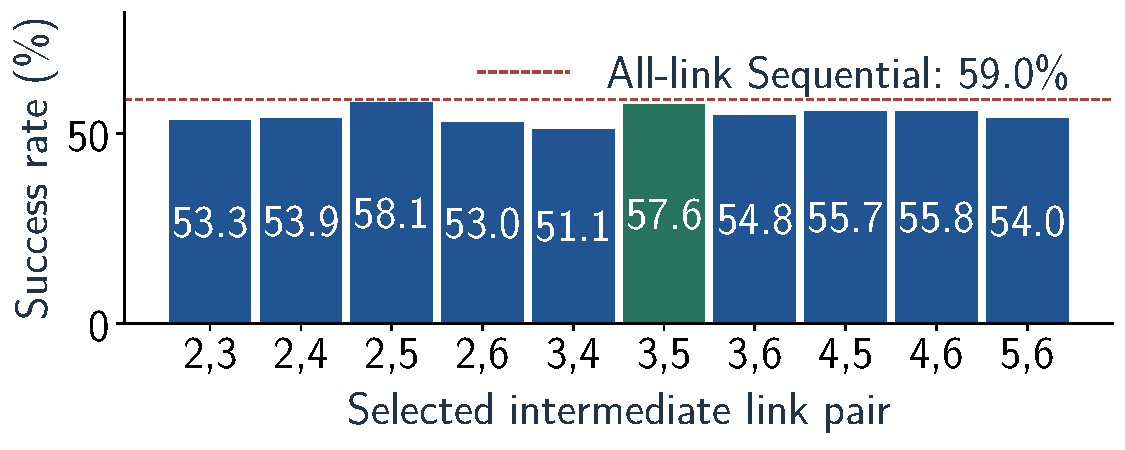
\includegraphics[width=.98\linewidth,height=43mm,keepaspectratio]{pair_variability.pdf}
    \begin{itemize}
      \item 10-pair mean: 54.73\%
      \item Best single pair on Validation: $(2,5)$, 58.10\%
      \item At least one successful pair: 820/1,000 episodes (oracle 82.00\%)
    \end{itemize}


  \end{slidebody}
\end{frame}

\begin{frame}{A3. Spatial Manipulator IK: Soft-Min Safety Term}
  \hypertarget{appendix-a3}{}
  \framesubtitle{3.4.1 Multi-Start IK with a Safety-Aware Null-Space Update}
  \begin{slidebody}
    \normalsize
    \[H_\tau(q)=-\tau\log\sum_r e^{-h_r^{\mathrm{IK}}(q)/\tau},\qquad
      \nabla H_\tau=\sum_r\pi_r\nabla h_r^{\mathrm{IK}}\]
    \[\pi_r=\frac{e^{-h_r^{\mathrm{IK}}/\tau}}{\sum_j e^{-h_j^{\mathrm{IK}}/\tau}},\qquad
      v_h=k_h(I-J^\dagger J)\nabla H_\tau\]
    \begin{block}{Orthogonal null-space projector $N=I-J^\dagger J$~\cite{siciliano2009robotics}}
      \[Jv_h=0,\qquad \nabla H_\tau^\top v_h=k_h\norm{N\nabla H_\tau}^2\geq0\]
      Nonnegative first-order change from the secondary term
    \end{block}
    \vfill
    \begin{itemize}
      \item Before clipping: zero EE twist from $v_h$; primary term also included
      \item IK iterates: neither an executed path nor a safety proof for all iterations
      \item No solution within the search budget; no proof of unreachability
    \end{itemize}
    \vfill
  \end{slidebody}
\end{frame}

\begin{frame}{A4. RDF Barriers: Differentiating Both Links' Motion}
  \hypertarget{appendix-a4}{}
  \framesubtitle{3.4.3 RDF-Based Construction of CBF}
  \begin{slidebody}
    \setlength{\abovedisplayskip}{3pt}\setlength{\belowdisplayskip}{3pt}
    \centering Fixed selected query set; $J_{x,k}$: query-point Jacobian\par\vfill
    \begin{align*}
      \xi_{ab,k}            & =R_b^\top(x_{a,k}-p_b),\qquad d_k=\tilde d_b(\xi_{ab,k}),             \\[1mm]
      J_{\xi,k}             & =R_b^\top\big(J_{x,k}-J_{p,b}+[x_{a,k}-p_b]_\times J_{\omega,b}\big), \\[1mm]
      \nabla_qh_{ab}^{\top} & =\sum_k\pi_k\nabla_\xi\tilde d_b(\xi_{ab,k})^\top J_{\xi,k},          \\[1mm]
      \pi_k                 & =\frac{e^{-\beta d_k}}{\sum_{j=1}^K e^{-\beta d_j}},\qquad K>1.
    \end{align*}\vfill
    \textbf{Soft-min approximation bound}~\cite{molnar2023composing}\par
    \[\min_kd_k-\varepsilon_{\mathrm{sm}}\leq D_{ab}\leq\min_kd_k,
      \quad\beta=\frac{\log K}{\varepsilon_{\mathrm{sm}}}\]\vfill
    No bound on RDF error or unqueried surface clearance\par\vfill
  \end{slidebody}
\end{frame}

\begin{frame}{A5. Stage-Transition Rules: Planar and Spatial Manipulator}
  \hypertarget{appendix-a5}{}
  \framesubtitle{3.3.4 Stage-Transition Rule}
  \begin{slidebody}
    \begin{tabularx}{\linewidth}{@{}l@{\hspace{4mm}}>{\raggedright\arraybackslash}X>{\raggedright\arraybackslash}X@{}}\toprule
      Condition         & Planar                                                                  & Spatial Manipulator                                                   \\\midrule
      \shortstack[l]{Link                                                                                                                                                 \\subtask} & Link 1 and 2 positions & Selected-link pose \\[3mm]
      Stage reached     & Link-position error within tolerance                                    & $\norm{e_{\mathrm p,i}}\leq0.05$ m; $\norm{\epsilon_i}\leq0.05$       \\[3mm]
      Stall condition   & Link subtask: small $\norm{u}$ near boundary $\Rightarrow$ next subtask & Low applied speed and insufficient progress $\Rightarrow$ termination \\[3mm]
      QP infeasible     & Link subtask: switch and recompute                                      & Termination before integration                                        \\[3mm]
      Numerical failure & Separate from infeasibility switching                                   & Termination                                                           \\\bottomrule
    \end{tabularx}\vfill
  \end{slidebody}
\end{frame}

\begin{frame}{A6. Paired Test Comparisons}
  \hypertarget{appendix-a6}{}
  \framesubtitle{4.2.5 Recovery Through Learned Link Selection}
  \begin{slidebody}
    \takeaway{No additional speed gain observed over the 10-pair mean}
    \normalsize
    \begin{tabularx}{\linewidth}{@{}Xrr@{}}\toprule
      Comparison (second $-$ first)               & Gap (pp)  & 95\% CI (pp)   \\\midrule
      Direct $\to$ All-link Sequential            & +9.70\,pp & $[6.00,13.40]$ \\[2mm]
      All-link Sequential $\to$ Learned selection & +5.70\,pp & $[2.70,8.60]$  \\[2mm]
      10-pair mean $\to$ Learned selection        & +5.70\,pp & $[3.74,7.65]$  \\\bottomrule
    \end{tabularx}\par\vspace{3mm}
    \centering Paired mean time: reference $\to$ Learned selection\par\vspace{3mm}
    \begin{tabularx}{\linewidth}{@{}Xrr@{}}\toprule
      Reference           & Success in both      & Mean time (s)   \\\midrule
      All-link Sequential & 467 episodes         & $47.97\to36.62$ \\[2mm]
      10-pair mean        & 4,792 episode--pairs & $36.05\to36.20$ \\\bottomrule
    \end{tabularx}


  \end{slidebody}
\end{frame}

\begin{frame}[allowframebreaks=0.88]{A7. References}
  \hypertarget{appendix-a7}{}
  \framesubtitle{Bibliography}
  \normalsize
  \bibliographystyle{IEEEtran}
  \bibliography{references}
\end{frame}

\begin{frame}{A8. Training Loss and Model Selection}
  \hypertarget{appendix-a8}{}
  \framesubtitle{3.5.4 Training Objective and Sequence Selection}
  \begin{slidebody}
    \normalsize
    \[\omega_k=\frac{e^{a_k}}{\sum_j e^{a_j}},\qquad
      \ell_{\mathrm{sel},n}=\begin{cases}
        -\log\sum_{k\in\mathcal K_n^+}\omega_k, & \mathcal K_n^+\ne\varnothing, \\
        0,                                      & \text{all pairs fail}.
      \end{cases}\]
    \[\mathcal L=\frac1{N_{\mathrm{tr}}}\sum_n\left[\frac1{10}\sum_k
        \ell(y_{nk},\hat p_k)+\lambda_{\mathrm{sel}}\ell_{\mathrm{sel},n}\right]\]
    \vfill
    \centering $\mathcal K_n^+=\{k:y_{nk}=1\}$,\quad $\lambda_{\mathrm{sel}}=3$\par\vfill
    \begin{itemize}
      \item AdamW: learning rate $10^{-3}$, weight decay $10^{-4}$, batch 64
      \item Up to 500 epochs, patience 50; five seeds: 11, 23, 37, 53, 71
      \item Selection by Validation successes, then BCE: seed 11, epoch 20
      \item Train-only joint normalization; all 10 outcomes per episode in one split
      \item Training: mixed legacy/revised QP data; Validation/Test: legacy controller
    \end{itemize}

    \vfill
  \end{slidebody}
\end{frame}

\begin{frame}{A9. Subtask Switching and Safe-Set Invariance}
  \hypertarget{appendix-a9}{}
  \framesubtitle{3.2 Sequential Kinematic Control Framework}
  \begin{slidebody}
    \takeaway{Conditional safety; no guarantee of goal convergence}
    \begin{block}{Assumptions for CBF invariance~\cite{ames2017cbf}}
      \begin{itemize}\setlength{\itemsep}{1mm}
        \item $C^1$ collision and joint-limit barriers
        \item $q(0)\in\mathcal C$; absolutely continuous $q(t)$
        \item Actual velocity satisfying all CBF inequalities almost everywhere
        \item Finitely many subtask switches; no state or barrier reset
      \end{itemize}
    \end{block}\vfill
    \[\begin{aligned}
        h_r(t)     & \geq e^{-\gamma_rt}h_r(0)\geq0,     \\[1mm]
        h_j^\pm(t) & \geq e^{-\alpha_jt}h_j^\pm(0)\geq0.
      \end{aligned}\]
    \centering $h_j^-=q_j-q_{j,\min},\quad h_j^+=q_{j,\max}-q_j$\par\vfill
    Separate checks for QP feasibility, convergence, and discretization\par\vfill
  \end{slidebody}
\end{frame}

\begin{frame}{A10. Planar Episode 30: Configurations and CLFs}
  \hypertarget{appendix-a10}{}
  \framesubtitle{4.1.2 Paired Outcomes and an Illustrative Trajectory}
  \begin{slidebody}
    \centering
    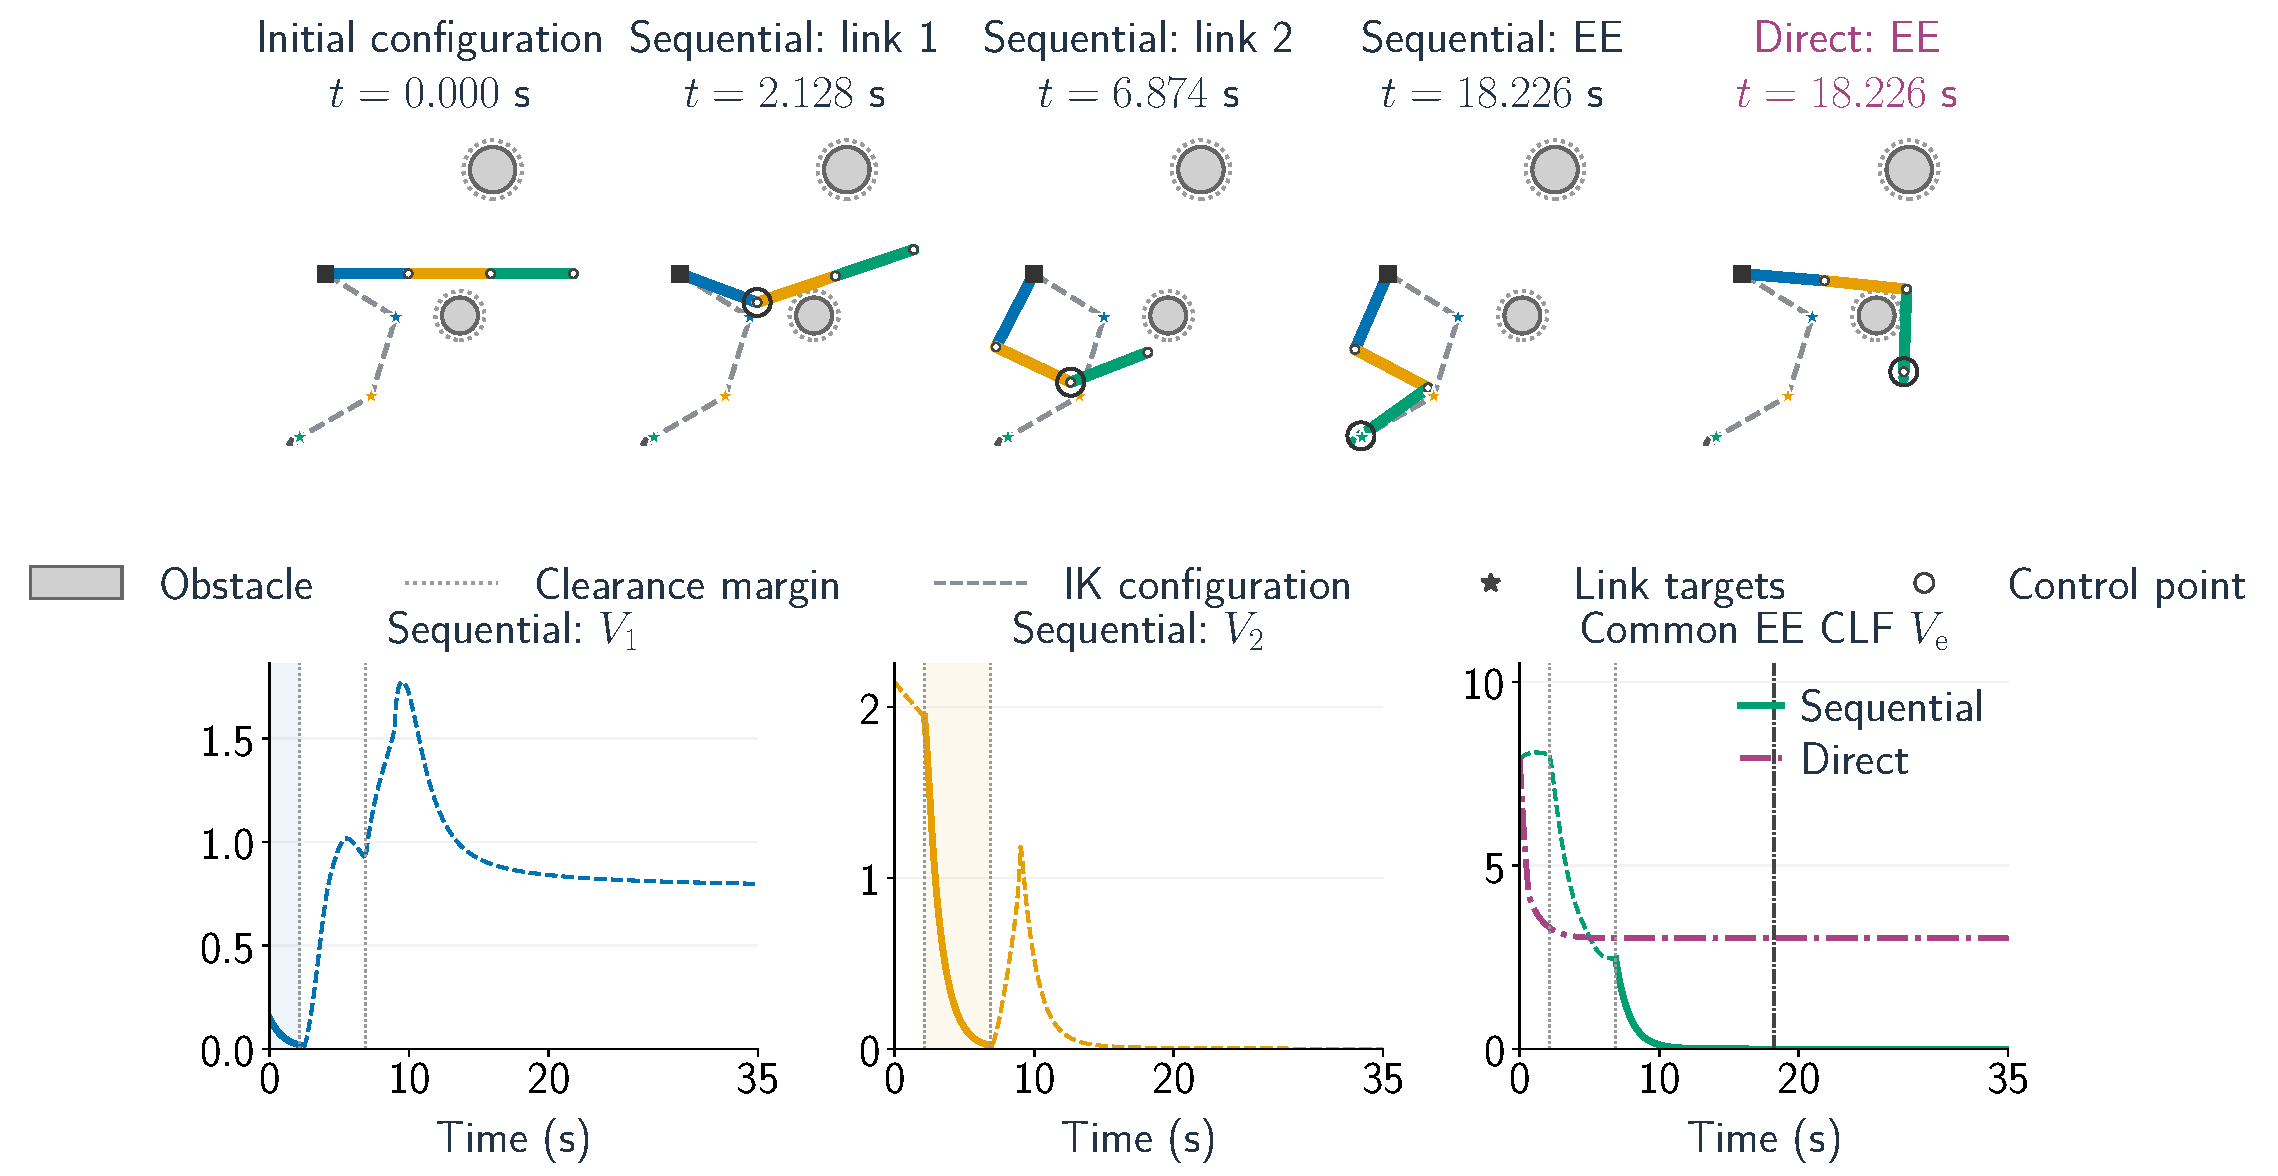
\includegraphics[width=\linewidth,height=68mm,keepaspectratio]{case030_overview.pdf}\par
    \vfill
  \end{slidebody}
\end{frame}

\begin{frame}{A11. Problem Definition and Goal Criteria}
  \hypertarget{appendix-a11}{}
  \framesubtitle{3.1 Problem Formulation}
  \begin{slidebody}
    \begin{block}{Joint-Velocity Kinematic Control}
      \[\dot q=u,\qquad q\in\R^n,\quad u:\text{joint velocity}\]
    \end{block}
    \vfill
    \begin{columns}[T,onlytextwidth]
      \column{.47\textwidth}
      \textbf{Inputs}
      \begin{itemize}\setlength{\itemsep}{3mm}
        \item Initial configuration $q_0$
        \item EE goal $(p_{\mathrm d},R_{\mathrm d})$
        \item Obstacles, joint limits, time $T_{\mathrm d}$
      \end{itemize}
      \column{.49\textwidth}
      \textbf{Goal criteria}
      \[\norm{e_{\mathrm p}}\leq\delta_{\mathrm p}\]
      \[\norm{e_{\mathrm o}}\leq\delta_{\mathrm o}\]
    \end{columns}
    \vfill
    \[\mathcal C=\{q:q_{\min}\leq q\leq q_{\max},\quad h_r(q)\geq0\ \forall r\}\]
    \centering $e_{\mathrm p}=p_{\ee}-p_{\mathrm d}$; spatial $e_{\mathrm o}=\epsilon_{\ee}$\par
    \vfill

  \end{slidebody}
\end{frame}

\begin{frame}{A12. Common CLF--CBF QP}
  \hypertarget{appendix-a12}{}
  \framesubtitle{3.2.2 CLF-CBF QP-Based Kinematic Control}
  \begin{slidebody}
    \takeaway{Hard CBF constraints; separate feasibility and convergence checks}
    \setlength{\abovedisplayskip}{4pt}\setlength{\belowdisplayskip}{4pt}
    \begin{align*}
      (u^*,\delta^*)=\argmin_{u,\delta}\quad
       & \tfrac12u^\top W_{\mathrm{u}} u+\tfrac12w_\delta\delta^2 \\[1mm]
      \text{subject to}\quad
       & \nabla_q V_i^\top u\leq-c_iV_i+\delta,                   \\[1mm]
       & \nabla_q h_r^\top u\geq-\gamma_rh_r,\quad r=1,\ldots,B,  \\[1mm]
       & -\alpha_j(q_j-q_{j,\min})\leq u_j
      \leq\alpha_j(q_{j,\max}-q_j),                               \\[1mm]
       & v_{\min,j}\leq u_j\leq v_{\max,j},\quad j=1,\ldots,n.
    \end{align*}
    \vfill
    $\delta$: CLF slack; $\alpha_j$: joint-limit CBF gain\par\vspace{2mm}
    $\subtask{s}$: $i=i_s$ for link stages; $V_{\ee}$ for final $\regtask$\par\vfill
    \centering QP solver: OSQP~\cite{stellato2020osqp}
  \end{slidebody}
\end{frame}

\begin{frame}{A13. Overall Control Architecture}
  \hypertarget{appendix-a13}{}
  \framesubtitle{3.2 Sequential Kinematic Control Framework}
  \begin{slidebody}
    \centering\sequentialframework\par\vfill
  \end{slidebody}
\end{frame}

\begin{frame}{A14. Interpreting the Reported Results}
  \hypertarget{appendix-a14}{}
  \framesubtitle{4.2.6 Interpretation and Limitations}
  \begin{slidebody}
    \begin{block}{Main comparison: 10-pair mean}
      Learned gain: $+5.70$\,pp / 95\% CI $[3.74,7.65]$\,pp
    \end{block}
    \vfill
    \begin{block}{Additional reference: Train-best fixed pair $(3,5)$}
      Highest Train success; Test success: 58.70\%\par\vspace{1mm}
      Learned gain: $+2.20$\,pp / 95\% CI $[-0.30,4.70]$\,pp
    \end{block}\vfill
    \textbf{Gain over the train-best fixed pair remains uncertain}\par\vfill
    \begin{block}{Recorded limitations}
      \begin{itemize}\setlength{\itemsep}{1.5mm}
        \item Test partition inspected during model development
        \item Approximate geometry and sampled-state collision checks
        \item Legacy controller: recorded QP residual violations
      \end{itemize}
    \end{block}\vfill

  \end{slidebody}
\end{frame}

\begin{frame}{A15. Episode-Wise Gain over the Pair Mean}
  \hypertarget{appendix-a15}{}
  \framesubtitle{4.2.5 Recovery Through Learned Link Selection}
  \begin{slidebody}
    \centering
    $d_e=y_{e,\hat k(e)}-\frac1{10}\sum_{k=1}^{10}y_{e,k}$\par\vspace{2mm}
    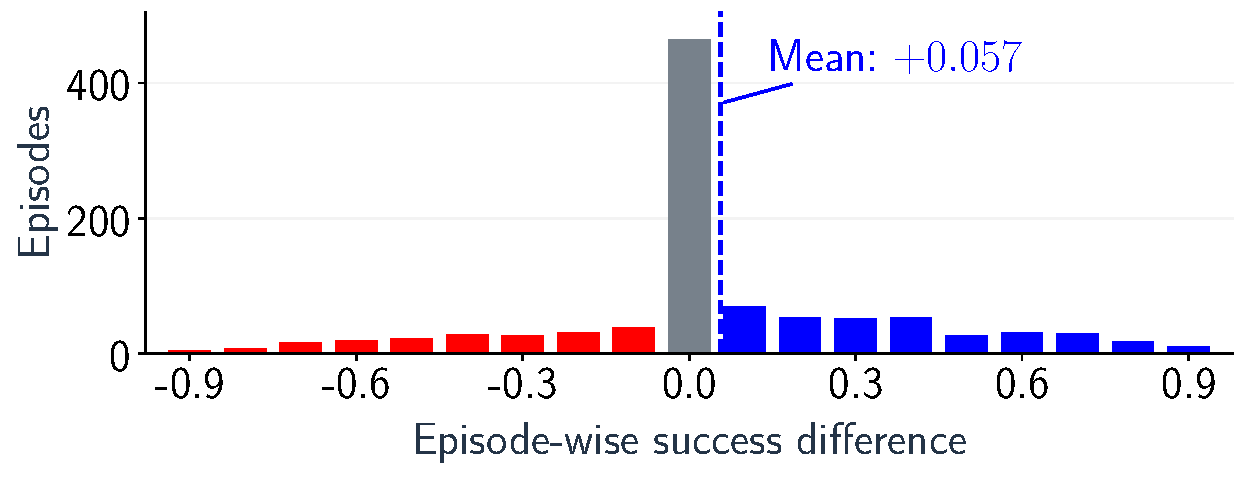
\includegraphics[width=\linewidth,height=42mm,keepaspectratio]{selection_gain_pair_mean.pdf}\par\vfill
    Mean gain: $+5.70$\,pp / 95\% CI $[3.74,7.65]$\,pp\par\vspace{2mm}
    Paired bootstrap over 1,000 episodes\par\vfill

  \end{slidebody}
\end{frame}

\begin{frame}{A16. Direct Episode: Stagnation near the Safety Boundary}
  \hypertarget{appendix-a16}{}
  \framesubtitle{2.3.1 Local Minima and Deadlock in CLF-CBF QP}
  \begin{slidebody}
    \centering
    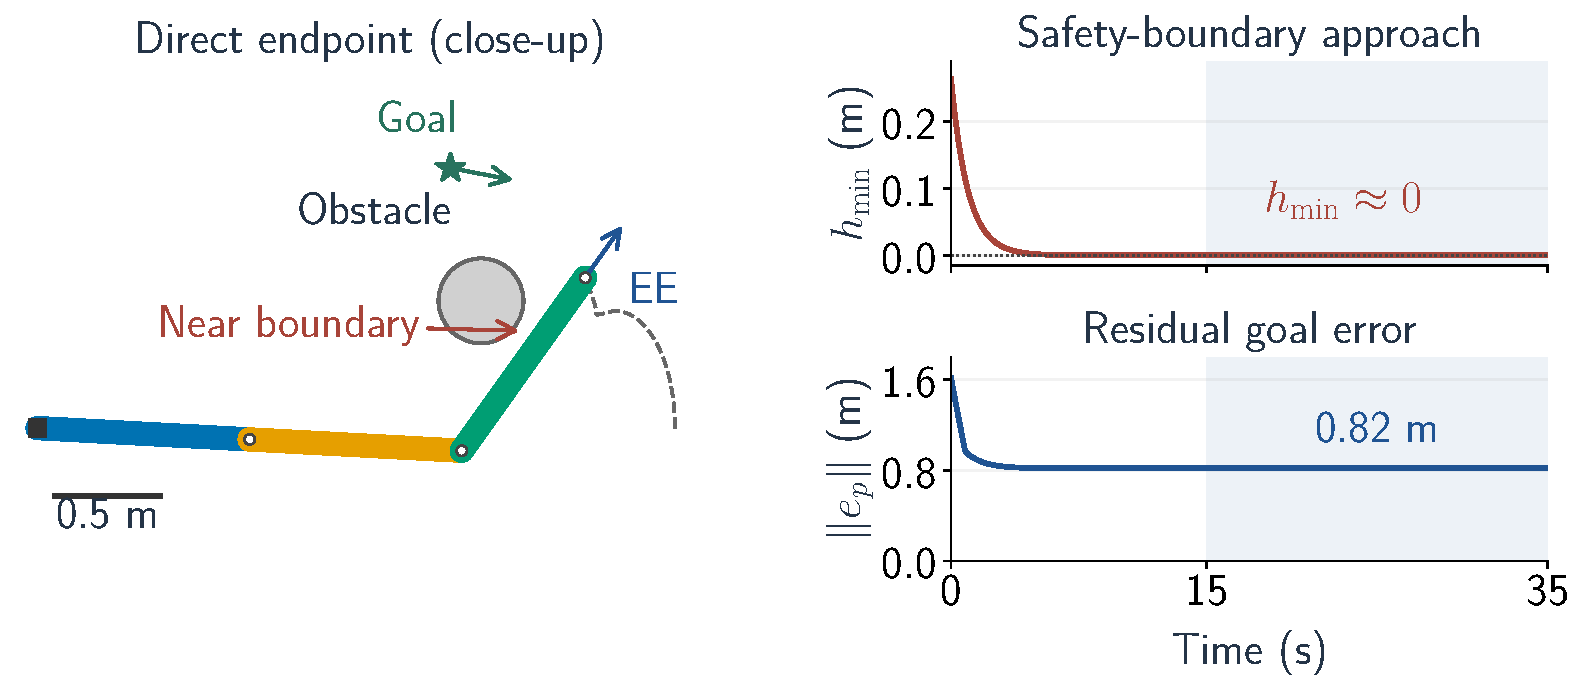
\includegraphics[width=\linewidth,height=45mm,keepaspectratio]{case180_boundary_stall.pdf}\par
    \vfill
    \begin{itemize}\setlength{\itemsep}{2mm}
      \item Episode 180: position error 0.82 m / vanishing speed
      \item Time-limit termination without QP infeasibility
    \end{itemize}

  \end{slidebody}
\end{frame}

\begin{frame}{A17. Related Work: Systems and Dimension Assumptions}
  \hypertarget{appendix-a17}{}
  \framesubtitle{2.3.1 Local Minima and Deadlock in CLF-CBF QP}
  \begin{slidebody}
    \begin{block}{General controller modifications}
      Reis: CLF shaping / Tan: nominal-input QP reformulation
    \end{block}\vfill
    \begin{block}{Gon\c{c}alves: circulation in configuration space}
      Basic theory: even $n$, $\Omega^\top=-\Omega$, $\Omega^\top\Omega=I$\\[2mm]
      Odd-dimensional extension: singular $\Omega$; additional feasibility concern\\[2mm]
      Demonstrations: 4-DOF arm and 15-dimensional multi-robot system
    \end{block}\vfill
    \begin{block}{This work: IK-derived link subtasks}
      Planar $q\in\mathbb R^3$ and spatial $q\in\mathbb R^7$\\[2mm]
      No even-dimension condition in the subtask-construction procedure
    \end{block}
  \end{slidebody}
\end{frame}

\end{document}
